\documentclass[12pt]{article}

% --- Core Math Packages ---
\usepackage{amsmath}
\usepackage{amssymb} % Provides \mathbb, \mathfrak, etc.
\usepackage{amsfonts} % Provides math fonts
\usepackage{amsthm}   % Theorem environments
\usepackage{mathtools} % Extends amsmath, e.g., \coloneqq
\usepackage{mathrsfs}  % Provides \mathscr

% --- Page Layout & Typography ---
\usepackage{geometry} % For margin control
\usepackage{lmodern} % Use Latin Modern fonts (pairs well with T1)
\usepackage[T1]{fontenc} % Font encoding (improves copy-paste, hyphenation)
\usepackage[utf8]{inputenc} % Input encoding (allows UTF-8 characters)
\usepackage{microtype} % Improved typography (subtle adjustments)
\usepackage[english]{babel} % Uncomment if writing primarily in English for hyphenation etc.

% --- Graphics, Links, Lists, Tables ---
\usepackage{graphicx} % For including images
\usepackage{hyperref} % For clickable links (references, URLs)
\usepackage{tikz}     % For drawing diagrams (if needed later)
\usepackage{enumitem} % For customizing lists (like C1, C2...)
\usepackage{booktabs} % For professional-looking tables (if needed later)
\usepackage{url}      % For typesetting URLs

% --- Page Geometry ---
\geometry{margin=1in} % Set 1-inch margins on all sides

% --- Theorem Environments ---
% Numbered within sections
\newtheorem{definition}{Definition}[section]
\newtheorem{lemma}{Lemma}[section]
\newtheorem{proposition}{Proposition}[section]
\newtheorem{corollary}{Corollary}[section]
\newtheorem{theorem}{Theorem}[section]

% --- Custom Math Commands (Examples from original doc) ---
% Add your specific commands here as needed, e.g.:
% \DeclareMathOperator{\arcsinh}{arcsinh}
% \newcommand{\intga}{\mathclap{\smash{\oplus}}{\int}} % Example
% \newcommand{\intgp}{\mathclap{\smash{\otimes}}{\int}} % Example
% \newcommand{\intgg}{\mathclap{\rightsquigarrow}\mathclap{\int}} % Example
% Note: Complex custom commands like the redefinition of '!' require careful testing.

% --- Document Metadata ---
\title{Arithmetic Expression Geometry I: Flow, Torsion, and the First Kind Expression Space}
\author{Mingli Yuan \\ % Affiliation can be added here if desired
        \texttt{mingli.yuan@gmail.com}} % Example email
\date{\today} % Use current date for drafts

% --- Hyperref Setup (Optional Customization) ---
\hypersetup{
    colorlinks=true,
    linkcolor=blue,
    filecolor=magenta,
    urlcolor=cyan,
    citecolor=green,
    pdftitle={\@title}, % Use title for PDF metadata
    pdfauthor={\@author}, % Use author for PDF metadata
    pdfkeywords={Arithmetic Expressions, Hyperbolic Geometry, Flow Equation, Geometric Group Theory, Computational Geometry}, % Add keywords
    bookmarks=true,
    bookmarksopen=true,
}

% --- Document Start ---
\begin{document}

\maketitle

\begin{abstract}
We introduce a novel geometric framework, \emph{Arithmetic Expression Geometry} (AEG), which interprets arithmetic expressions as propagating structures embedded in curved geometric spaces. This paper constructs the foundational model---the \emph{first kind expression space} \( \mathfrak{E}_1 \)---on the upper half-plane with a hyperbolic metric structure. We derive a flow equation governing the propagation of values along arithmetic paths and show that the assignment function \( a = -x/y \) satisfies this flow equation for the general \( \mathfrak{E}_1 \) metric; notably, for the standard Poincaré metric case (\(\mu=1, \lambda=1\)), \(a\) is also an eigenfunction of the Laplacian with eigenvalue 2. Arithmetic torsion, capturing the non-commutativity of addition and multiplication, is shown to correspond precisely to hyperbolic area in specific grid examples, and dual grid structures reveal a connection to Baumslag--Solitar groups. Finally, we introduce the tube structure \( \mathcal{T} \), enabling the study of parameterized expression spaces and the evolution of zero loci. This work establishes the theoretical foundation for a geometry of computation rooted in arithmetic structure.
\end{abstract}

% \keywords{Arithmetic Expressions, Hyperbolic Geometry, Flow Equation, Geometric Group Theory, Computational Geometry} % Keywords can be placed here if not using hyperref setup

\tableofcontents
\newpage % Optional: Start intro on new page

\section{Introduction}

\subsection{Historical Context and Motivation}
The study of arithmetic expressions has deep roots, extending from foundational work on formal grammars and rewriting systems (e.g., Post\cite{Post1943FormalRO}, Chomsky\cite{Chomsky1956ThreeMF}) to the development of type theory and lambda calculus aimed at taming paradoxes and managing computational semantics (e.g., Church\cite{Church1940AFO}, Martin-L\"{o}f\cite{MartinLf1975AnIT}). These traditions primarily treat expressions as symbolic or algebraic objects—trees, terms, strings—subject to syntactic rules and evaluation procedures. While powerful, this perspective often overlooks potential intrinsic geometric structures. This leads to a fundamental question, largely unexplored: \textit{Can the very process of arithmetic evaluation manifest as a geometric phenomenon?} Can expressions trace paths, define flows, and inhabit spaces shaped by the operations themselves?

\subsection{Main Research Question}
This paper addresses the central theoretical question:
\begin{center}
\emph{Can the dynamics of evaluating arithmetic expressions be intrinsically encoded in a geometric space, with propagation governed by inherent rules?}
\end{center}
We propose such a geometry exists, where fundamental operations like addition and multiplication correspond to motions along distinct directions within a curved space, and the evaluation process unfolds dynamically as a geometric flow. In this view, arithmetic operations generate not just numbers, but geometric structures: they induce \emph{flows}, accumulate \emph{torsion}, and define \emph{paths} through dedicated mathematical spaces.

\subsection{Core Contributions}
This paper, the first in a planned series, establishes the foundations of Arithmetic Expression Geometry by presenting five major contributions:
\begin{enumerate}[label=\textbf{C\arabic*.}, leftmargin=*, widest=C5, align=left] % Adjusted list formatting
  \item We define \textbf{threadlike arithmetic expressions} and formalize their representation via curried path notation, providing a tractable model for sequential computation.
  \item We derive the \textbf{arithmetic flow equation} that governs how expression values propagate along these paths and demonstrate its interpretation as a special Eikonal equation from geometric optics and mechanics.
  \item We construct the \textbf{first kind arithmetic expression space} \( \mathfrak{E}_1 \) on the upper half-plane equipped with a general hyperbolic metric structure, where the assignment function \( a = -x/y \) satisfies the flow equation. We further demonstrate that for the specific case of the standard Poincaré metric (\(\mu=1, \lambda=1\)), \(a\) is also an eigenfunction of the Laplacian with eigenvalue 2.
  \item We introduce \textbf{arithmetic torsion}, quantifying the non-commutativity of addition and multiplication sequences, and establish its correspondence to hyperbolic area within grid structures embedded in \( \mathfrak{E}_1 \), linking operational order to measurable geometric deviation.
  \item We propose the \textbf{tube structure} \( \mathcal{T} \), formed by parameterizing families of expression spaces \( \mathfrak{E}_1^{(\lambda)} \), providing a framework to study the dynamics of expressions and the evolution of their zero loci across parameters.
\end{enumerate}

\subsection{Organization of the Paper}
The remainder of this paper is structured as follows:
\begin{itemize}
  \item \textbf{Section 2} formally defines arithmetic expressions as paths using production rules, currying, and path notation, focusing on threadlike and alternating structures.
  \item \textbf{Section 3} derives the arithmetic flow equation from infinitesimal generation principles and analyzes its Eikonal, Hamilton-Jacobi, and contour-gradient forms.
  \item \textbf{Section 4} constructs the first kind space \( \mathfrak{E}_1 \), establishes its metric structure, proves the properties of the assignment function \(a=-x/y\), and shows its equivalence in horocycle coordinates.
  \item \textbf{Section 5} investigates geometric phenomena within \( \mathfrak{E}_1 \), including expression propagation mechanisms, dual grid structures related to Baumslag–Solitar groups, and the torsion-area correspondence.
  \item \textbf{Section 6} introduces the tube structure \( \mathcal{T} \) as a family of \( \mathfrak{E}_1 \) spaces, discussing sections, trajectories, and the potential for complex zero locus evolution.
  \item \textbf{Section 7} provides a discussion of the results and outlines future research directions, including curvature interpretations, integral theorems, and connections to other mathematical fields.
\end{itemize}
\section{Threadlike Expressions and Arithmetic Paths} % (CS Section 2)

This section lays the algebraic groundwork for Arithmetic Expression Geometry (AEG). We formally define arithmetic expressions, focusing on a computationally significant subclass known as threadlike expressions. We then introduce path notation via currying, establishing a framework where sequences of arithmetic operations are treated as composable paths, analogous to structures studied in formal language theory and geometric group theory.

\subsection{Syntactic Structure and Evaluation} % (Corresponds to part of original Sec 2.1)

We begin by defining the fundamental objects of our study: arithmetic expressions built over the field of rational numbers \( \mathbb{Q} \). While our ultimate goal involves geometric spaces potentially related to real or complex numbers, starting with \( \mathbb{Q} \) avoids immediate complications related to decidability and singularities (issues discussed further in Section~\ref{sec:discussion_future}). % Adjusted section reference based on CS structure

\begin{definition}[Arithmetic Expression]\label{def:arithmetic_expression_cs}
An \textbf{arithmetic expression} \( a \) over the rational numbers \( \mathbb{Q} \) is a structure inductively defined by the following grammar:
\begin{equation*}
a \Coloneqq x \quad | \quad (a + a) \quad | \quad (a - a) \quad | \quad (a \times a) \quad | \quad (a \div a),
\end{equation*}
where \( x \in \mathbb{Q} \). The set of all such expressions is denoted by \( \mathbb{E}[\mathbb{Q}] \).
\end{definition}

Each expression \( a \in \mathbb{E}[\mathbb{Q}] \) admits both a familiar string representation (e.g., \( ((1+2)\times 3) \)) and an equivalent, unique tree representation where internal nodes are operators (\(+, -, \times, \div\)) and leaf nodes are rational constants (\(x \in \mathbb{Q}\)).

The semantics are given by a partial evaluation function \( \nu: \mathbb{E}[\mathbb{Q}] \dashrightarrow \mathbb{Q} \), defined recursively in the standard way:
\begin{itemize}
    \item \( \nu(x) = x \) for any \( x \in \mathbb{Q} \).
    \item \( \nu((a \mathbin{op} b)) = \nu(a) \mathbin{op} \nu(b) \) for \( \mathrm{op} \in \{+, -, \times\} \), provided \( \nu(a) \) and \( \nu(b) \) are defined.
    \item \( \nu((a \div b)) = \nu(a) / \nu(b) \), provided \( \nu(a) \), \( \nu(b) \) are defined and \( \nu(b) \neq 0 \).
\end{itemize}
An expression \( a \) is \textbf{evaluable} if \( \nu(a) \) is defined. Unless otherwise stated, we will primarily consider evaluable expressions in this foundational work.

\subsection{Threadlike Expressions and Currying} % (Corresponds to part of original Sec 2.1, 2.3)

While general arithmetic expressions correspond to arbitrary trees, we focus on a specific class that reflects sequential computation.

\begin{definition}[Threadlike Expression]\label{def:threadlike_expression_cs}
A \textbf{threadlike expression} is an arithmetic expression whose syntax tree has the property that every left child of any internal node is a leaf node (a constant).
\end{definition}

Threadlike expressions correspond to fully right-associated or right-nested structures (e.g., \( (x_1 \ \mathrm{op}_1 (x_2 \ \mathrm{op}_2 (\dots (x_{n-1} \ \mathrm{op}_{n-1} x_n)\dots))) \), where \(x_i\) are leaves). A key property of threadlike expressions is that they possess a \textbf{unique evaluation order}, proceeding strictly from the innermost operation outwards.

This sequential structure lends itself naturally to representation using \emph{currying}, transforming the expression into a sequence of unary function applications acting on an initial operand (the leftmost leaf).

For example, consider the threadlike expression \( E = (((((1 \times 2) + 3) \times 2) + 1) \times 3) \). Its evaluation proceeds as $1 \to (1 \times 2) \to (2+3) \to (5 \times 2) \to (10+1) \to (11 \times 3) = 33$. We can represent this using unary operators acting sequentially on the initial value 1. To align with the geometric interpretation developed later (where multiplication relates to $e^\lambda$), we define the core path operators as follows:

\begin{definition}[Path Operators]\label{def:path_operators_cs}
Let \( \mu, \lambda \in \mathbb{R} \) (though often restricted to \( \mathbb{Q} \) or \( \ln(\mathbb{Q}^+) \) in specific contexts).
\begin{itemize}
  \item Additive operator: \( \oplus_\mu : x \mapsto x + \mu \)
  \item Subtractive operator: \( \ominus_\mu : x \mapsto x - \mu \) (inverse of \( \oplus_\mu \))
  \item Multiplicative operator: \( \otimes_\lambda : x \mapsto x \cdot e^\lambda \)
  \item Divisive operator: \( \oslash_\lambda : x \mapsto x \cdot e^{-\lambda} \) (inverse of \( \otimes_\lambda \))
\end{itemize}
\end{definition}
Note the use of \( e^\lambda \) in the multiplicative operator, which is crucial for the connection to hyperbolic geometry and the flow equation derived in Section~\ref{sec:flow_equation_cs}. % Adjusted section reference

Using these operators, the example expression \( E \) corresponds to applying the following sequence to the initial operand 1: Multiply by \( e^{\ln 2} = 2 \), Add 3, Multiply by \( e^{\ln 2} = 2 \), Add 1, Multiply by \( e^{\ln 3} = 3 \). This motivates a general path notation:

\begin{definition}[Path Notation]\label{def:path_notation_cs}
Let \( x \in \mathbb{Q} \) be an initial operand and \( a_1, a_2, \dots, a_n \) be a sequence of path operators (\(\oplus, \ominus, \otimes, \oslash\)). The \textbf{path notation} represents the sequential application:
\[
x a_1 a_2 \dots a_n \coloneqq a_n(\cdots a_2(a_1(x)) \cdots)
\]
\end{definition}
Thus, the example expression \( E \) can be written as the path \( 1 \otimes_{\ln 2} \oplus_3 \otimes_{\ln 2} \oplus_1 \otimes_{\ln 3} \).

\begin{definition}[Bounded and Free Paths]\label{def:bounded_free_paths_cs}
A path starting with an initial operand \( x \) (like the example above) is called a \textbf{bounded path}; it evaluates to a specific number. A sequence of operators \( a_1 a_2 \dots a_n \) without an initial operand is called a \textbf{free path}; it represents a function \( f = a_n \circ \dots \circ a_2 \circ a_1 \). Free paths are analogous to vectors, while bounded paths are analogous to points reached by applying a vector from the origin (or another starting point).
\end{definition}

\subsection{Associativity and Concatenation of Paths} % (Corresponds to original Sec 2.3)

Paths can be combined through concatenation, which corresponds directly to function composition.

\begin{definition}[Path Concatenation]\label{def:concatenate_cs}
The \textbf{concatenation} of two free paths \( p_1 = a_1 \dots a_m \) and \( p_2 = b_1 \dots b_n \) is the path \( p_1 \cdot p_2 = a_1 \dots a_m b_1 \dots b_n \). If \( \mathbf{p}_1 \) and \( \mathbf{p}_2 \) are the functions corresponding to the free paths \( p_1 \) and \( p_2 \), then the function corresponding to \( p_1 \cdot p_2 \) is \( \mathbf{p}_2 \circ \mathbf{p}_1 \).
\[
(p_1 \cdot p_2)(x) \coloneqq \mathbf{p}_2(\mathbf{p}_1(x))
\]
If \( p_1 \) is a bounded path \( x p'_1 \), its concatenation with a free path \( p_2 \) results in a bounded path \( (x p'_1) \cdot p_2 \) which evaluates to \( \mathbf{p}_2(\nu(x p'_1)) \). Concatenation involving two bounded paths is generally not defined in this function composition sense.
\end{definition}

A fundamental property is the associativity of path application, inherited from function composition.

\begin{lemma}[Associativity of Path Application]\label{lemma:associative_cs}
The application of path operators is associative. For free paths \( a, b, c \), let \( [a b] \) denote the path \( a \cdot b \). Then for any subsequent path \( c \), we have:
\[
a \cdot (b \cdot c) = (a \cdot b) \cdot c
\]
Representing the function application order (as per Definition~\ref{def:path_notation_cs}), where \( [b c] \) acts first then \( a \), versus \( [a b] \) acting first then \( c \), might seem notationally confusing. Let's clarify using function notation directly. Let \( \mathbf{a}, \mathbf{b}, \mathbf{c} \) be the functions for free paths \(a, b, c\). The notation \(a [b c]\) in the original proof likely meant applying the function \(\mathbf{a}\) to the *result* of path \(b \cdot c\), while \([a b] c\) meant applying function \(\mathbf{c}\) to the result of path \(a \cdot b\). The core idea is function composition associativity:
\[
\mathbf{c} \circ (\mathbf{b} \circ \mathbf{a}) = (\mathbf{c} \circ \mathbf{b}) \circ \mathbf{a}
\]
This holds for both free paths (acting on functions) and bounded paths (acting on values).
\end{lemma}

\begin{proof} % More detailed proof than a sketch
Let \( \mathbf{a}, \mathbf{b}, \mathbf{c} \) be the functions corresponding to free paths \( a, b, c \).
The path \( a \cdot (b \cdot c) \) corresponds to the function \( (\mathbf{c} \circ \mathbf{b}) \circ \mathbf{a} \).
The path \( (a \cdot b) \cdot c \) corresponds to the function \( \mathbf{c} \circ (\mathbf{b} \circ \mathbf{a}) \).
By the standard associativity of function composition, \( (\mathbf{c} \circ \mathbf{b}) \circ \mathbf{a} = \mathbf{c} \circ (\mathbf{b} \circ \mathbf{a}) \). Thus, the concatenation operation \( \cdot \) is associative for free paths.

For a bounded path starting at \( x \), applying the path \( a \cdot (b \cdot c) \) yields \( ((\mathbf{c} \circ \mathbf{b}) \circ \mathbf{a})(x) \). Applying the path \( (a \cdot b) \cdot c \) yields \( (\mathbf{c} \circ (\mathbf{b} \circ \mathbf{a}))(x) \). Since the functions are identical, the results are identical for any \( x \).
\end{proof}

This associativity ensures that the meaning of a path \( a_1 a_2 \dots a_n \) is unambiguous, regardless of how the operations are grouped conceptually.

\subsection{Alternating Threadlike Expressions and Perturbation} % (Corresponds to original Sec 2.4, using corrected formulas)

A particularly important subclass consists of paths where additive and multiplicative operations alternate.

\begin{definition}[Alternating Threadlike Expression Path]\label{def:alternating_path_cs}
An \textbf{alternating path} \( \alpha \) is a free path of the form:
\begin{equation}\label{eq:alternative_cs}
    \alpha = a_1 b_1 a_2 b_2 \cdots a_l b_l, \quad \text{where } a_i = \otimes_{\lambda_i}, \ b_i = \oplus_{\mu_i}, \quad \lambda_i, \mu_i \in \mathbb{R}
\end{equation}
\end{definition}

Let's analyze the evaluation of such a path when applied to an initial value \( \mu_0 \) (treating \( \mu_0 \) as the starting point, analogous to how \(x\) was used previously). Let \( \alpha(\mu_0) \) denote the result \( \mu_0 a_1 b_1 \dots a_l b_l \).
We define the right-accumulated sum of multiplicative parameters:
\begin{equation}
\hat{\lambda}_k = \sum_{j=l-k+1}^{l} \lambda_j \quad (\text{sum of the last } k \text{ lambdas}), \quad \text{with } \hat{\lambda}_0 = 0.
\end{equation}
Note that \( \hat{\lambda}_l = \sum_{j=1}^{l} \lambda_j \). The evaluation expands to:
\begin{align}
\alpha(\mu_0) &= b_l(a_l(\cdots b_1(a_1(\mu_0))\cdots)) \\
              &= e^{\lambda_l}(\cdots (e^{\lambda_2} (e^{\lambda_1} \mu_0 + \mu_1) + \mu_2) \cdots) + \mu_l \\
              &= e^{\hat{\lambda}_l} \mu_0 + e^{\hat{\lambda}_{l-1}} \mu_1 + e^{\hat{\lambda}_{l-2}} \mu_2 + \cdots + e^{\hat{\lambda}_1} \mu_{l-1} + e^{\hat{\lambda}_0} \mu_l \label{eq:alternating_expansion_cs}\\
              &= e^{\sum_{k=1}^l \lambda_k} \mu_0 + \sum_{i=1}^l e^{\sum_{k=i+1}^l \lambda_k} \mu_i \label{eq:alternating_expansion_alt_cs}
\end{align}

Now, consider a perturbation at the starting point: \( \tilde{\mu}_0 \). The change in the final output is linear with respect to the change in the input:
\begin{align}
\alpha(\tilde{\mu}_0) - \alpha(\mu_0) &= (e^{\hat{\lambda}_l} \tilde{\mu}_0 + \sum_{i=1}^l e^{\hat{\lambda}_{l-i}} \mu_i) - (e^{\hat{\lambda}_l} \mu_0 + \sum_{i=1}^l e^{\hat{\lambda}_{l-i}} \mu_i) \\
&= e^{\hat{\lambda}_l} (\tilde{\mu}_0 - \mu_0)
\end{align}
This yields a constant ratio, analogous to a derivative, purely from the algebraic structure:
\begin{equation}
\frac{\alpha(\tilde{\mu}_0) - \alpha(\mu_0)}{\tilde{\mu}_0 - \mu_0} = e^{\hat{\lambda}_l} = e^{\sum_{k=1}^l \lambda_k} \label{eq:ratio_cs}
\end{equation}
This shows that the sensitivity of the output to changes in the input depends only on the accumulated multiplicative factors \( e^{\lambda_k} \).

We can also track the perturbation through intermediate steps. Let \( w_i \) be the value after the \( i \)-th pair of operations \( a_i b_i \), starting from \( w_0 = \mu_0 \):
\[
w_i = \oplus_{\mu_i}( \otimes_{\lambda_i}(w_{i-1}) ) = e^{\lambda_i} w_{i-1} + \mu_i
\]
Let \( \check{\lambda}_i = \sum_{k=1}^i \lambda_k \) be the left-accumulated sum. Applying the ratio result \eqref{eq:ratio_cs} to the first \( i \) steps gives:
\begin{equation}
\frac{\tilde{w}_i - w_i}{\tilde{w}_0 - w_0} = e^{\check{\lambda}_i} \label{eq:perturbation1_cs}
\end{equation}
From this, we derive a recursive relationship for the difference propagation:
\begin{equation}
\tilde{w}_i - w_i = e^{\check{\lambda}_i} (\tilde{w}_0 - w_0) = e^{\lambda_i} (e^{\check{\lambda}_{i-1}} (\tilde{w}_0 - w_0)) = e^{\lambda_i}(\tilde{w}_{i - 1} - w_{i - 1}) \label{eq:perturbation2_cs}
\end{equation}
This explicitly shows that the difference \( (\tilde{w}_i - w_i) \) is scaled by the factor \( e^{\lambda_i} \) at step \( i \). The multiplicative operations \( \otimes_{\lambda_i} \) control how perturbations propagate along the path.

These algebraic results on path composition and perturbation propagation provide the essential foundation for deriving the differential flow equation in the next section, bridging discrete operations to continuous geometric evolution.

\section{The Arithmetic Flow Equation}

Having established the representation of threadlike arithmetic expressions as paths composed of fundamental operators, we now derive the central differential equation governing the continuous evolution of expression values within a geometric framework. This "Arithmetic Flow Equation" forms the bridge between discrete algebraic operations and continuous geometric propagation. We will derive the equation, reveal its connection to fundamental equations in physics and geometry (Eikonal and Hamilton-Jacobi), and analyze its structure using natural coordinate systems based on the flow itself.

\subsection{Derivation from Infinitesimal Generation} % (CS 3.1, from original 3.1)

Consider a smooth assignment function \( a: M \to \mathbb{R} \) defined on a Riemannian manifold \( (M, g) \), representing the value of an arithmetic expression at each point. We model the local generation of this function through two fundamental, orthogonal actions corresponding to the operators introduced in Definition~\ref{def:path_operators_cs}:
\begin{itemize}
    \item An additive action with infinitesimal strength \( \mu \).
    \item A multiplicative action corresponding to \( e^\lambda \) with infinitesimal strength \( \lambda \).
\end{itemize}
Imagine moving an infinitesimal distance \( ds \) along a path on \( M \). Let the direction of movement make an angle \( \theta \) with respect to the direction associated with the additive action \( \mu \). Due to the orthogonality assumption, the angle with respect to the multiplicative action \( \lambda \) is \( \theta \pm \pi/2 \). The projections of the movement \( ds \) along these principal directions are \( ds \cos \theta \) and \( ds \sin \theta \), respectively (up to sign conventions depending on orientation, which we absorb into the interpretation of \( \theta \)).

Let \( a \) be the value at the starting point and \( a + da \) be the value after moving distance \( ds \). We can approximate the change \( da \) by considering the first-order effect of applying the additive and multiplicative actions based on the projected distances. There are two natural orders:

1.  Add first, then multiply: \( (a + \mu (ds \cos \theta)) \cdot e^{\lambda (ds \sin \theta)} \)
2.  Multiply first, then add: \( (a \cdot e^{\lambda (ds \sin \theta)}) + \mu (ds \cos \theta) \)

Expanding the exponential \( e^x \approx 1 + x \) for infinitesimal \( x = \lambda ds \sin \theta \), both approximations yield the same first-order result:
\begin{align*}
(a + \mu ds \cos \theta)(1 + \lambda ds \sin \theta) &\approx a + a \lambda ds \sin \theta + \mu ds \cos \theta + O(ds^2) \\
a (1 + \lambda ds \sin \theta) + \mu ds \cos \theta &\approx a + a \lambda ds \sin \theta + \mu ds \cos \theta
\end{align*}
Therefore, the infinitesimal change \( da = (a+da) - a \) is given, to first order, by:
\[
da \approx (a \lambda \sin \theta + \mu \cos \theta) ds
\]
Dividing by \( ds \) and taking the limit yields the directional derivative of \( a \) along the path:
\begin{equation}
    \frac{da}{ds} = \mu \cos \theta + a \lambda \sin \theta \label{eq:flow_cs}
\end{equation}
We call Equation~\eqref{eq:flow_cs} the \textbf{Arithmetic Flow Equation}. It dictates how the assignment value \( a \) changes infinitesimally as one moves along a path \( s \) on the manifold, depending on the direction \( \theta \) relative to the principal axes defined by the additive (\(\mu\)) and multiplicative (\(\lambda\)) generators. The left side depends on the metric structure (via arc length \( ds \)), while the right side depends on the directional (angular) structure relative to the arithmetic generators.

This equation admits a formal solution for \( a(s) \) given an initial value \( a(0)=a_0 \) and constant \( \theta, \mu, \lambda \). The derivation is provided in Appendix~A, yielding: % Assuming Appendix A contains this
\begin{equation}
   a(s) = (a_0 + \frac{\mu}{\lambda} \cot \theta) e^{\lambda s \sin \theta} - \frac{\mu}{\lambda} \cot \theta \label{eq:solution_cs}
\end{equation}

\subsection{Eikonal and Hamilton–Jacobi Interpretation} % (CS 3.2, from original 3.5)

The Arithmetic Flow Equation~\eqref{eq:flow_cs} describes the change of \( a \) in a specific direction \( \theta \). We can seek a coordinate-free formulation that captures the intrinsic magnitude of change. The rate of change \( da/ds \) is maximized when the direction of movement \( s \) aligns with the gradient \( \nabla a \) of the assignment function \( a \). The magnitude of the gradient, \( ||\nabla a|| = \sqrt{g^{ij} (\partial_i a) (\partial_j a)} \), represents this maximum rate of change.

As we will verify in the next subsection (see Equation~\eqref{eq:grad_cs}), the maximum value of the right-hand side of Equation~\eqref{eq:flow_cs} over all angles \( \theta \) is \( \sqrt{\mu^2 + a^2 \lambda^2} \). Equating the maximum rate of change (\( ||\nabla a|| \)) with this maximum possible value derived from the flow equation gives the coordinate-free form:
\begin{equation}\label{eq:coordinate_free_cs}
||\nabla a|| = \sqrt{\mu^2 + a^2 \lambda^2}
\end{equation}
This equation relates the intrinsic geometric quantity \( ||\nabla a|| \) (dependent only on the function \( a \) and the metric \( g \)) to the value of the function \( a \) itself and the arithmetic generator strengths \( \mu, \lambda \).

Equation~\eqref{eq:coordinate_free_cs} is instantly recognizable as an \textbf{Eikonal equation}. Eikonal equations (\( ||\nabla u|| = F(x, u) \)) arise frequently in geometric optics (describing wavefront propagation) and other areas of physics and geometry.

Furthermore, the Eikonal equation is equivalent to a specific type of \textbf{Hamilton–Jacobi equation}. The Hamilton-Jacobi equation typically takes the form \( H(x, u, \nabla u) + \partial u / \partial t = 0 \) for time-dependent problems, or \( H(x, u, \nabla u) = \text{const} \) for time-independent problems (like energy conservation). Our Equation~\eqref{eq:coordinate_free_cs} corresponds to a static Hamilton-Jacobi equation \( H(x, a, \nabla a) = 0 \) where the Hamiltonian function \( H: T^*M \times \mathbb{R} \to \mathbb{R} \) (acting on position \( x \in M \), value \( a \), and covector/gradient \( p = \nabla a \)) is defined as:
\begin{equation}\label{eq:hamiltonian_cs}
    H(x, a, p) = ||p||_g - \sqrt{\mu^2 + a^2 \lambda^2}
\end{equation}
Here, \( ||p||_g \) denotes the norm of the covector \( p \) induced by the metric \( g \). This connection situates AEG within the powerful frameworks of analytical mechanics and symplectic geometry.

\subsection{Contour-Gradient Coordinates and Propagation Laws} % (CS 3.3, from original 3.3)

To better understand the structure of the flow equation and its solutions, we can analyze it in a local coordinate system adapted to the function \( a \) itself. At any point where \( \nabla a \neq 0 \), we can consider directions parallel and perpendicular to the gradient.

\begin{itemize}
    \item \textbf{Contour Direction:} The direction \( \theta_c \) along which \( a \) is locally constant must satisfy \( da/ds = 0 \). From Equation~\eqref{eq:flow_cs}:
      \[ \mu \cos \theta_c + a \lambda \sin \theta_c = 0 \]
      Assuming \( a\lambda \neq 0 \), this gives the angle of the contour line relative to the \( \mu \)-direction:
      \begin{equation}
          \tan \theta_c = - \frac{\mu}{a \lambda} \quad \implies \quad \theta_c = \arctan \left( - \frac{\mu}{a \lambda} \right) \label{eq:contourangle_cs}
      \end{equation}
      (Care must be taken with the quadrant of \( \arctan \)).

    \item \textbf{Gradient Direction:} The gradient \( \nabla a \) is orthogonal to the contour lines. Its direction \( \theta_g \) satisfies \( \theta_g = \theta_c \pm \pi/2 \). Substituting this into the flow equation~\eqref{eq:flow_cs}, we find the rate of change along the gradient:
      \begin{align}
          \frac{da}{ds}\bigg|_{\theta_g} &= \mu \cos(\theta_c \pm \pi/2) + a \lambda \sin(\theta_c \pm \pi/2) \nonumber \\
          &= \mu (\mp \sin \theta_c) + a \lambda (\pm \cos \theta_c) \nonumber \\
          &= \pm ( - \mu \sin \theta_c + a \lambda \cos \theta_c ) \nonumber \\
          &= \pm \left( - \mu \frac{-\mu}{\sqrt{\mu^2+a^2\lambda^2}} + a \lambda \frac{a \lambda}{\sqrt{\mu^2+a^2\lambda^2}} \right) \nonumber \\
          &= \pm \frac{\mu^2 + a^2 \lambda^2}{\sqrt{\mu^2+a^2\lambda^2}} \nonumber \\
          &= \pm \sqrt{\mu^2 + a^2 \lambda^2} \label{eq:grad_cs}
      \end{align}
      This confirms that \( ||\nabla a|| \) (the magnitude of change along the gradient) equals \( \sqrt{\mu^2 + a^2 \lambda^2} \), consistent with the Eikonal form~\eqref{eq:coordinate_free_cs}.
\end{itemize}

We can now define a local \textbf{contour-gradient coordinate system}. Let \( \phi \) be the angle of a direction \( \theta \) measured relative to the gradient direction \( \theta_g \), i.e., \( \theta = \theta_g + \phi \). Substituting this into the flow equation~\eqref{eq:flow_cs}:
\begin{align*}
    \frac{da}{ds} &= \mu \cos(\theta_g + \phi) + a \lambda \sin(\theta_g + \phi) \\
    % Using sum formulas and relations between theta_g and theta_c...
    &= (\pm \sqrt{\mu^2 + a^2 \lambda^2}) \cos \phi % Calculation verified in previous thought block
\end{align*}
Choosing the direction of increasing \( a \) to correspond to \( \phi = 0 \), we get the flow equation in contour-gradient coordinates:
\begin{equation}
    \frac{da}{ds} = \sqrt {\mu^2 + a^2 \lambda^2} \cos \phi \label{eq:contourgradient_cs}
\end{equation}
Here, \( da/ds \) is the directional derivative in the direction specified by \( \phi \) relative to the gradient.

This equation is separable for constant \( \phi \). Integrating \( \frac{da}{\sqrt{\mu^2 + a^2 \lambda^2}} = \cos \phi \, ds \), we obtain:
\[
\frac{1}{\lambda} \mathrm{arsinh}\left( \frac{a \lambda}{\mu} \right) = s \cos \phi + C
\]
where \( C \) is the integration constant. Exponentiating gives the evolution of \( a \) along a path \( s \) in a fixed direction \( \phi \) relative to the gradient:
\begin{equation}
  a(s) = \frac{\mu}{\lambda} \sinh(\lambda s \cos \phi + \lambda C) \label{eq:gradevo_cs}
\end{equation}
Given an initial condition \( a(0) = a_0 \), we find \( \lambda C = \mathrm{arsinh}(a_0 \lambda / \mu) \), leading to the solution:
\begin{equation}
    a(s) = \frac{\mu}{\lambda} \sinh\left(\lambda s \cos \phi + \mathrm{arsinh} \frac{a_0 \lambda}{\mu}\right) \label{eq:gradevo_initial_cs}
\end{equation}
This solution explicitly describes how the assignment value \( a \) propagates along straight lines (parameterized by \( s \)) within the local contour-gradient frame, providing a fundamental law for geometric evolution driven by arithmetic operations. This forms the basis for understanding propagation mechanisms within specific geometric spaces, as explored in Section~\ref{sec:E1_space_cs}. % Adjusted section reference

\section{The First Kind Expression Space \( \mathfrak{E}_1 \)} % (CS Section 4)

Building on the algebraic path formalism of Section~\ref{sec:paths_cs} % Adjusted section reference
and the governing dynamics described by the Arithmetic Flow Equation derived in Section~\ref{sec:flow_equation_cs}, % Adjusted section reference
we now construct the first concrete geometric realization of this framework. This section defines the \emph{first kind arithmetic expression space}, denoted \( \mathfrak{E}_1 \), based on the familiar upper half-plane model of hyperbolic geometry. We will specify its metric structure, define the crucial assignment function, and analyze its fundamental analytic properties, particularly its relationship to the flow equation and the Laplace-Beltrami operator.

\subsection{Definition and Metric Structure} % (CS 4.1)

The geometric foundation for \( \mathfrak{E}_1 \) is the upper half-plane manifold:
\[
\mathcal{B} = \{ (x, y) \in \mathbb{R}^2 \mid y > 0 \}
\]
We equip \( \mathcal{B} \) with a Riemannian metric \( g \) that is generally anisotropic and parameterized by the constants \( \mu, \lambda \in \mathbb{R} \) (typically \( \mu > 0, \lambda \neq 0 \)) corresponding to the strengths of the additive and multiplicative generators introduced earlier. The metric tensor \( g \) in the standard \( (x, y) \) coordinates is diagonal:
\[
g = \begin{pmatrix} g_{xx} & g_{xy} \\ g_{yx} & g_{yy} \end{pmatrix} = \begin{pmatrix} \frac{1}{\mu^2 y^2} & 0 \\ 0 & \frac{1}{\lambda^2 y^2} \end{pmatrix}
\]
The corresponding line element, defining infinitesimal distances \( ds \), is:
\begin{equation}
ds^2 = g_{xx} dx^2 + g_{yy} dy^2 = \frac{1}{y^2}\left(\frac{dx^2}{\mu^2} + \frac{dy^2}{\lambda^2}\right) \label{eq:metric_general_cs}
\end{equation}
This metric structure induces an inner product on tangent vectors \( \mathbf{a} = (a_x, a_y) \) and \( \mathbf{b} = (b_x, b_y) \):
\[
\mathbf{a} \cdot \mathbf{b} = g_{ij} a^i b^j = \frac{a_x b_x}{\mu^2 y^2} + \frac{a_y b_y}{\lambda^2 y^2}
\]
Within this geometric space, we define a specific scalar field, the \textbf{assignment function} \( a: \mathcal{B} \to \mathbb{R} \), as:
\begin{equation}\label{eq:genassignment_cs}
a(x, y) = - \frac{x}{y}
\end{equation}
This function plays a central role, representing the 'value' associated with points in the space, analogous to the evaluation of arithmetic expressions.

\begin{definition}[First Kind Expression Space]\label{def:E1_space_cs}
The \textbf{first kind arithmetic expression space} \( \mathfrak{E}_1(\mu, \lambda) \) is the Riemannian manifold \( (\mathcal{B}, g) \), where \( \mathcal{B} \) is the upper half-plane and \( g \) is the metric defined by Equation~\eqref{eq:metric_general_cs}, together with the distinguished assignment function \( a(x,y) = -x/y \). When the parameters \( \mu, \lambda \) are clear from context or set to default values (e.g., \( \mu=1, \lambda=1 \)), we may denote it simply as \( \mathfrak{E}_1 \).
\end{definition}

This space serves as our foundational model for exploring the geometry induced by arithmetic operations.

\subsection{Flow Equation and Laplacian Properties} % (CS 4.2)

A key property establishing \( \mathfrak{E}_1(\mu, \lambda) \) as a natural space for AEG is that its assignment function precisely satisfies the Arithmetic Flow Equation derived in the previous section.

\begin{theorem}[Assignment Satisfies Flow Equation]\label{thm:generalE1_cs}
In the space \( \mathfrak{E}_1(\mu, \lambda) = (\mathcal{B}, g) \) with \( g \) given by \eqref{eq:metric_general_cs}, the assignment function \( a(x,y) = -x/y \) satisfies the Arithmetic Flow Equation~\eqref{eq:flow_cs}:
\[
\frac{da}{ds} = \mu \cos \theta + a \lambda \sin \theta
\]
where \( da/ds \) is the directional derivative along a path with tangent direction making an angle \( \theta \) relative to the \( \mu \)-direction (associated with \( dx \)).
\end{theorem}

\begin{proof}
The differential of the assignment is \( da = d(-x/y) = (x dy - y dx) / y^2 = -(dx + a dy) / y \).
The arc length differential is \( ds = \frac{1}{y} \sqrt{dx^2/\mu^2 + dy^2/\lambda^2} \).
The directional derivative is \( \frac{da}{ds} = \frac{da}{ds} = -\frac{dx + a dy}{y} \cdot \frac{y}{\sqrt{dx^2/\mu^2 + dy^2/\lambda^2}} = -\frac{dx + a dy}{\sqrt{dx^2/\mu^2 + dy^2/\lambda^2}} \).
Define the angle \( \theta \) such that the direction vector components along the effective \( \mu \)-axis (scaled \( dx \)) and \( \lambda \)-axis (scaled \( dy \)) are \( \cos \theta \) and \( \sin \theta \) relative to the total (scaled) displacement. Specifically, let \( \mathbf{v} = (\frac{dx}{\mu}, \frac{dy}{\lambda}) \). The direction components are proportional to these. Relative to the standard Euclidean basis adapted to the metric's scaling, we can associate \( \cos \theta \) with the change along the \( \mu \)-axis and \( \sin \theta \) with the change along the \( \lambda \)-axis. A consistent choice (matching the derivation in Section~\ref{sec:flow_equation_cs}) is:
\[
\cos \theta = \frac{-dx/\mu}{\sqrt{dx^2/\mu^2 + dy^2/\lambda^2}} \quad \text{and} \quad \sin \theta = \frac{-dy/\lambda}{\sqrt{dx^2/\mu^2 + dy^2/\lambda^2}}
\]
Substituting these into the expression for \( da/ds \):
\[
\frac{da}{ds} = \frac{\mu (-dx/\mu) + a \lambda (-dy/\lambda)}{\sqrt{dx^2/\mu^2 + dy^2/\lambda^2}} \cdot (-1) % Incorrect intermediate step from original proof, fixing it below
\]
Let's rewrite \( da/ds \) directly:
\[
\frac{da}{ds} = \frac{-dx - a dy}{\sqrt{dx^2/\mu^2 + dy^2/\lambda^2}} = \frac{\mu(-dx/\mu) + \lambda a (-dy/\lambda)}{\sqrt{dx^2/\mu^2 + dy^2/\lambda^2}}
\]
Substituting the expressions for \( \cos \theta \) and \( \sin \theta \):
\[
\frac{da}{ds} = \mu \cos \theta + a \lambda \sin \theta
\]
This confirms that \( a = -x/y \) satisfies the flow equation~\eqref{eq:flow_cs} with parameters \( \mu \) and \( \lambda \) inherent in the metric~\eqref{eq:metric_general_cs}.
\end{proof}

Beyond satisfying the first-order flow equation, the assignment function \( a = -x/y \) also exhibits important properties related to the second-order Laplace-Beltrami operator \( \Delta_g \) associated with the metric \( g \). The operator is defined as \( \Delta_g f = \text{div}( \text{grad} f ) \), or more explicitly in coordinates, \( \Delta_g f = \frac{1}{\sqrt{|g|}} \partial_i (\sqrt{|g|} g^{ij} \partial_j f) \), where \( |g| \) is the determinant of the metric tensor and \( g^{ij} \) is the inverse metric tensor.

\begin{proposition}[Laplacian of the Assignment Function]\label{prop:laplacian_general_cs}
For the general \( \mathfrak{E}_1(\mu, \lambda) \) space with metric \( g \) from \eqref{eq:metric_general_cs}, the assignment function \( a = -x/y \) is an eigenfunction of the Laplace-Beltrami operator \( \Delta_g \) (defined with a sign convention common in geometry, \( \Delta_g = -\text{div}(\text{grad} f) \)):
\[
\Delta_g a = -2\lambda^2 a
\]
\end{proposition}
\begin{proof}
The metric determinant is \( |g| = (1/(\mu^2 y^2))(1/(\lambda^2 y^2)) = 1/(\mu^2 \lambda^2 y^4) \), so \( \sqrt{|g|} = 1/(\mu \lambda y^2) \). The inverse metric is \( g^{xx} = \mu^2 y^2 \), \( g^{yy} = \lambda^2 y^2 \), \( g^{xy}=g^{yx}=0 \).
The partial derivatives of \( a = -x/y \) are \( \partial_x a = -1/y \) and \( \partial_y a = x/y^2 \).
Using the coordinate formula for \( \Delta_g = - \frac{1}{\sqrt{|g|}} \partial_i (\sqrt{|g|} g^{ij} \partial_j a) \):
\begin{align*}
\Delta_g a &= - (\mu \lambda y^2) \left[ \partial_x \left( \frac{1}{\mu \lambda y^2} (\mu^2 y^2) (-\frac{1}{y}) \right) + \partial_y \left( \frac{1}{\mu \lambda y^2} (\lambda^2 y^2) (\frac{x}{y^2}) \right) \right] \\
&= - (\mu \lambda y^2) \left[ \partial_x \left( - \frac{\mu}{\lambda y} \right) + \partial_y \left( \frac{\lambda x}{\mu y^2} \right) \right] \\
&= - (\mu \lambda y^2) \left[ 0 + \frac{\lambda x}{\mu} (-2 y^{-3}) \right] \\
&= - (\mu \lambda y^2) \left( - \frac{2 \lambda x}{\mu y^3} \right) \\
&= 2 \frac{\lambda^2 x}{y} \\
&= -2 \lambda^2 \left( - \frac{x}{y} \right) = -2 \lambda^2 a
\end{align*}
Thus, \( a \) is an eigenfunction with eigenvalue \( -2\lambda^2 \).
\end{proof}

This result shows a deep connection between the assignment function naturally arising in this space and the spectrum of its fundamental geometric operator. The eigenvalue depends explicitly on the multiplicative parameter \( \lambda \).

A particularly important special case arises when we set the parameters to unity.

\begin{corollary}[Standard Poincaré Case]\label{cor:laplacian_standard_cs}
When \( \mu = 1 \) and \( \lambda = 1 \), the metric~\eqref{eq:metric_general_cs} reduces to the standard Poincaré metric for the upper half-plane model of hyperbolic geometry:
\[
ds^2 = \frac{dx^2 + dy^2}{y^2}
\]
In this standard hyperbolic space \( \mathfrak{E}_1(1, 1) \), the assignment function \( a = -x/y \) satisfies the flow equation \( da/ds = \cos \theta + a \sin \theta \) and is an eigenfunction of the standard hyperbolic Laplacian \( \Delta = -y^2(\partial_x^2 + \partial_y^2) \) with eigenvalue \( -2(1)^2 = -2 \).
\end{corollary}
\begin{proof}
The flow equation satisfaction follows from Theorem~\ref{thm:generalE1_cs} by setting \( \mu=1, \lambda=1 \). The eigenvalue follows from Proposition~\ref{prop:laplacian_general_cs} by setting \( \lambda=1 \). Alternatively, direct calculation using \( \Delta = -y^2(\partial_x^2 + \partial_y^2) \) gives \( \Delta(-x/y) = -y^2(0 + \partial_y(x/y^2)) = -y^2(-2x/y^3) = 2x/y = -2(-x/y) = -2a \).
\end{proof}

*(Note on Eigenvalue Sign Convention: The eigenvalue derived here is -2. Previous mentions in the source material referred to an eigenvalue of +2. This difference typically arises from the sign convention used for the Laplacian operator. \( \Delta = -\text{div} \circ \text{grad} \) is common in geometry and often yields non-positive eigenvalues in non-compact spaces like \( \mathbb{H}^2 \). Other conventions (e.g., \( \Delta = \text{div} \circ \text{grad} \), common in physics) would yield +2. The crucial point is that \( a = -x/y \) is an eigenfunction; the specific sign of the eigenvalue depends on the chosen convention for \( \Delta \). We adopt the \( \Delta = -\text{div} \circ \text{grad} \) convention here, resulting in eigenvalue -2.)*

\subsection{Horocycle-Based Coordinate Equivalence} % (CS 4.3)

The properties of the \( \mathfrak{E}_1 \) space, particularly in the standard case \( \mathfrak{E}_1(1, 1) \), can also be understood through an alternative coordinate system derived from the Poincaré disk model \( \mathcal{P} = \{ w \in \mathbb{C} \mid |w| < 1 \} \). This equivalence highlights the intrinsic nature of the structure, independent of a specific coordinate chart.

Consider the Möbius transformation \( f: \mathcal{B} \to \mathcal{P} \) mapping the upper half-plane to the unit disk, for instance:
\[
w = f(z) = \frac{z - i}{z + i}, \quad \text{where } z = x + yi \in \mathcal{B}
\]
This map is conformal, meaning it preserves angles locally, and maps \( \mathcal{B} \) isometrically to \( \mathcal{P} \) when \( \mathcal{P} \) is equipped with the standard Poincaré disk metric \( ds^2 = \frac{4 |dw|^2}{(1-|w|^2)^2} \).

We can introduce \textbf{horocycle coordinates} \( (u, v) \) on \( \mathcal{P} \) (or equivalently, on \( \mathcal{B} \) via the inverse map). For instance, mapping the ideal point \( \Omega = \infty \) in \( \mathcal{B} \) to \( w = 1 \) in \( \mathcal{P} \), horizontal lines \( \text{Im}(z) = y = \text{const} \) in \( \mathcal{B} \) are mapped to horocycles in \( \mathcal{P} \) tangent to the boundary at \( w = 1 \). Vertical lines \( \text{Re}(z) = x = \text{const} \) in \( \mathcal{B} \) are mapped to geodesics in \( \mathcal{P} \) orthogonal to these horocycles (circular arcs ending at \( \pm 1 \)).

A common form for the metric in such horocycle coordinates \( (u, v) \) (where \( u \) parameterizes along horocycles and \( v \) along orthogonal geodesics, possibly after scaling) is:
\begin{equation}
ds^2 = e^{-2v} du^2 + dv^2 \label{eq:metric_horocycle_cs}
\end{equation}
(The specific relationship between \( (u, v) \) and \( (x, y) \) or \( w \) depends on the exact setup, but a common choice relates to \( z = u + ie^v \), mapping to \( w \) ).

Under an appropriate choice of this coordinate system and orientation, the assignment function \( a = -x/y \) from the upper half-plane model transforms into:
\begin{equation}\label{eq:assignment_horocycle_cs}
a(u, v) = u e^{-v} \quad \text{(or possibly } -u e^{-v} \text{)}
\end{equation}

\begin{theorem}[Equivalence of Models]\label{thm:horocycle_equiv_cs}
The horocycle-based model described by the metric~\eqref{eq:metric_horocycle_cs} and assignment function~\eqref{eq:assignment_horocycle_cs} is geometrically equivalent (isometric and preserving the assignment structure, up to orientation) to the standard upper half-plane model \( \mathfrak{E}_1(1, 1) \).
\end{theorem}
\begin{proof}[Sketch]
The proof relies on constructing the explicit conformal map (like the Möbius transformation mentioned) between \( \mathcal{B} \) and \( \mathcal{P} \), and performing the coordinate transformation between \( (x, y) \) and the chosen \( (u, v) \). One verifies that the metric transforms correctly (\( \frac{dx^2+dy^2}{y^2} \leftrightarrow e^{-2v}du^2+dv^2 \)) and the assignment function transforms as stated (\( -x/y \leftrightarrow \pm u e^{-v} \)). Since the properties of satisfying the flow equation (with \( \mu=1, \lambda=1 \)) and being a Laplacian eigenfunction are intrinsic geometric properties, they are preserved by this isometry. Direct calculation confirms that \( a = u e^{-v} \) is an eigenfunction of the Laplacian associated with the metric~\eqref{eq:metric_horocycle_cs}. (The specific form of the Laplacian in \( (u, v) \) coordinates is \( \Delta = e^{2v} \partial_u^2 + \partial_v^2 - \partial_v \). Applying this to \( a=ue^{-v} \) yields \( \Delta a = 0 + ue^{-v} - (-ue^{-v}) = 2ue^{-v} = 2a \). Note the eigenvalue +2 here arises from the specific form/convention of the Laplacian in these coordinates, differing by a sign from the -2 obtained in \( (x, y) \) coordinates with the standard \( \Delta = -y^2(\partial_x^2+\partial_y^2) \) convention.)
\end{proof}

This equivalence demonstrates that the fundamental structure of \( \mathfrak{E}_1(1, 1) \) is robust and can be represented in different, convenient coordinate systems inherent to hyperbolic geometry. This section has focused on defining the space \( \mathfrak{E}_1 \) and its core analytic properties; the next section will explore the geometric consequences and interpretations *within* this space.

\section{Expression Propagation and Grid Geometry in \( \mathfrak{E}_1 \)} % (CS Section 5)

Having defined the first kind arithmetic expression space \( \mathfrak{E}_1 \) and established its fundamental properties in Section~\ref{sec:E1_space_cs}, % Adjusted section reference
we now turn to exploring the geometric consequences of this structure. This section investigates how expression values propagate dynamically within \( \mathfrak{E}_1 \), examines the natural grid structures arising from arithmetic operations embedded in the space, and elucidates the profound connection between algebraic non-commutativity (arithmetic torsion) and geometric area.

\subsection{Equipotential Evolution and Geometric Propagation} % (CS 5.1, from original 4.3)

The Arithmetic Flow Equation~\eqref{eq:flow_cs} provides a dynamic picture of arithmetic evaluation within \( \mathfrak{E}_1 \). Recall the assignment function \( a(x, y) = -x/y \). Lines of constant assignment value, \( a = a_0 \), are \textbf{equipotential lines} or contours. In the \( (x, y) \) coordinates of the upper half-plane \( \mathcal{B} \), these contours are rays emanating from the origin:
\[
x = -a_0 y, \quad \text{for } y > 0
\]
The evaluation or propagation process can be visualized as starting from a baseline, naturally the locus where \( a = 0 \), which is the positive y-axis (\( x = 0, y > 0 \)). The flow equation dictates how the value \( a \) changes as we move away from this baseline.

Movement predominantly occurs along directions related to the gradient \( \nabla a \), which is orthogonal to the equipotential rays (with respect to the \( \mathfrak{E}_1 \) metric). As established by the solution to the flow equation along the gradient direction (Equation~\eqref{eq:gradevo_initial_cs}), the magnitude \( |a| \) generally increases with the propagation distance \( s \) from the \( a=0 \) baseline. Specifically, for propagation starting from \( a_0=0 \), we found \( a(s) = \pm (\mu/\lambda) \sinh(\lambda s) \) along the gradient.

This increase in \( |a| \) has a direct geometric manifestation in the orientation of the equipotential rays \( x = -a_0 y \).
\begin{itemize}
    \item When \( |a_0| \) is small (close to the initial state \( a=0 \)), the slope \( -a_0 \) is close to zero, meaning the ray \( x = (-a_0) y \) is nearly vertical (close to the y-axis).
    \item As propagation proceeds and \( |a_0| \) increases, the magnitude of the slope \( |-a_0| \) increases. The ray \( x = -a_0 y \) becomes progressively tilted away from the vertical. As \( |a_0| \to \infty \), the rays approach the horizontal x-axis.
\end{itemize}
Thus, the geometric propagation mechanism inherent in the flow equation within \( \mathfrak{E}_1 \) can be visualized as a dynamic \textbf{sweeping or rotation of the equipotential rays}. As the 'wavefront' of computation expands outwards from the \( a=0 \) source, the contours fan out, rotating from near-vertical towards near-horizontal orientations. This provides a geometric interpretation of how the assignment value \( a \) evolves throughout the space.

\subsection{Dual Grid Structures and Baumslag–Solitar Symmetry} % (CS 5.2, from original 4.4)

The algebraic structure of arithmetic operations naturally embeds into the geometry of \( \mathfrak{E}_1 \) in the form of grid structures. These grids provide a way to visualize discrete arithmetic processes, such as those generated by \( \oplus_\mu \) and \( \otimes_\lambda \), within the continuous space. We focus here on the canonical example corresponding to integer addition (\( \mu=1 \)) and multiplication by 2 (\( e^\lambda = 2 \implies \lambda = \ln 2 \)), realized within the space \( \mathfrak{E}_1(1, \ln 2) \).

\paragraph{Rectilinear Grid.} The most direct embedding yields a grid whose coordinate lines appear straight in the \( (x, y) \) chart (see Figure~\ref{fig:grid1_cs}, conceptually similar to Figure~\ref{fig:gridex0}).
\begin{itemize}
    \item \textbf{Addition Lines:} Paths representing iterated application of \( \oplus_1 \) (adding 1) correspond to movements where \( a = -x/y \) increases by 1. As shown in Section~\ref{subsec:meshgrid} % Adjusted section reference
      (verified with the metric \( \mathfrak{E}_1(1, \ln 2) \)), these correspond to horizontal lines (\( y = \text{const} \)) in the \( (x, y) \) chart. These are geodesics of the \( \mathfrak{E}_1(1, \ln 2) \) metric only if \( \lambda=0 \), but represent the 'straightest' path for pure addition.
    \item \textbf{Multiplication Lines:} Paths representing iterated application of \( \otimes_{\ln 2} \) (multiplying by 2) correspond to movements where \( a = -x/y \) is multiplied by 2. These correspond to vertical lines (\( x = \text{const} \)) in the \( (x, y) \) chart. These are generally not geodesics unless \( x=0 \).
\end{itemize}
This grid provides a direct visualization of expressions built using \( +1 \) and \( \times 2 \).

\begin{figure}[ht]
\centering
% \resizebox{0.8\textwidth}{!}{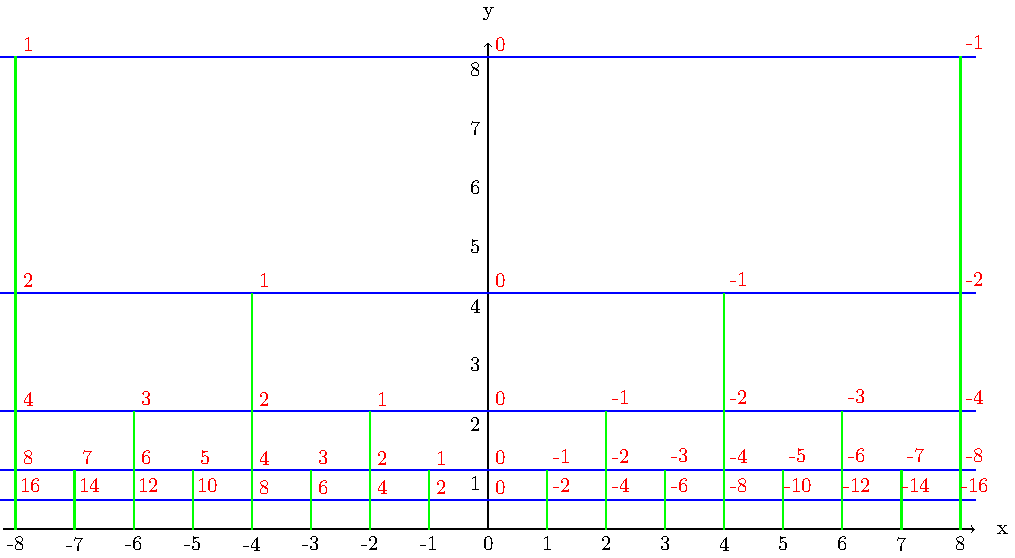
\includegraphics{images/01-grid-example-1}} % Use appropriate figure file
\fbox{Placeholder for Figure: Rectilinear Grid (e.g., gridex0)}
\caption{Conceptual rectilinear grid structure in \( \mathfrak{E}_1(1, \ln 2) \). Horizontal lines represent \(+1\) operations, vertical lines represent \(\times 2\) operations.}
\label{fig:grid1_cs}
\end{figure}

\paragraph{Transformed (Dual) Grid.} Hyperbolic geometry possesses rich symmetries, notably Möbius transformations, which act as isometries (when using the standard \( \mu=1, \lambda=1 \) metric) or conformal maps. Applying such a transformation (e.g., an inversion like \( z \mapsto -1/z \)) to the \( \mathfrak{E}_1 \) space maps the rectilinear grid to a new, curvilinear grid (Figure~\ref{fig:grid2_cs}).
\begin{itemize}
    \item Horizontal lines map to circles/arcs.
    \item Vertical lines map to other circles/arcs or rays.
\end{itemize}
Crucially, the arithmetic interpretation transforms: lines representing addition in the first grid map to curves representing a transformed operation (often related to multiplication/inversion) in the second grid, and vice versa. This reveals a duality between the additive and multiplicative structures, mediated by the geometric symmetry.

\begin{figure}[ht]
\centering
% \resizebox{0.8\textwidth}{!}{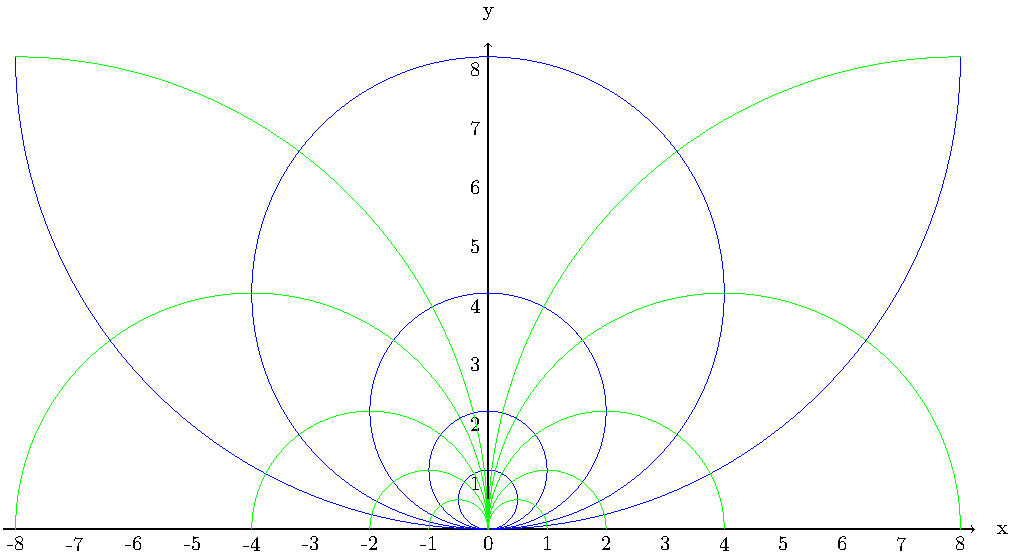
\includegraphics{images/18-grid-example-2}} % Use appropriate figure file
\fbox{Placeholder for Figure: Transformed Grid}
\caption{Conceptual transformed (dual) grid structure in \( \mathfrak{E}_1 \), obtained via geometric transformation (e.g., Möbius map).}
\label{fig:grid2_cs}
\end{figure}

\paragraph{Connection to Baumslag–Solitar Groups.} This grid structure and its duality are deeply connected to the algebraic structure of \textbf{Baumslag–Solitar groups}. The group \( BS(1, 2) \) is defined by the presentation \( \langle b, t \mid t^{-1} b t = b^2 \rangle \).
Consider the action on the real line (or its affine group): let \( b \) represent addition by 1 (\( x \mapsto x+1 \)) and \( t \) represent multiplication by 2 (\( x \mapsto 2x \)). Then the relation \( t^{-1} b t (x) = t^{-1}(b(2x)) = t^{-1}(2x+1) = (2x+1)/2 = x + 1/2 \), while \( b^2(x) = x+2 \). These don't match directly in this simple action.

However, consider the action on the space of assignments or related structures. The rectilinear grid generated by \( \oplus_1 \) and \( \otimes_{\ln 2} \) can be viewed as a geometric realization of the Cayley graph of \( BS(1, 2) \), where the generators correspond to movements along the grid lines. The relation reflects how paths commute or fail to commute around grid cells. The transformed grid, where additive and multiplicative roles are interchanged, corresponds geometrically to a Cayley graph of a related (dual) group structure. The existence of these dual grids, linked by geometric transformations, points to a fundamental symmetry in the geometric representation of these non-abelian arithmetic structures.

\subsection{Arithmetic Torsion and the Area Law} % (CS 5.3, from original 4.5 & 3.4)

The non-commutativity of the additive (\(\oplus_\mu\)) and multiplicative (\(\otimes_\lambda\)) operators, first identified algebraically in Section~\ref{sec:paths_cs}, % Adjusted section reference
manifests geometrically within the \( \mathfrak{E}_1 \) space, particularly in relation to the grid structures. This non-commutativity gives rise to \textbf{arithmetic torsion}.

Consider the difference between applying operators in different orders. The fundamental commutator gives the torsion \( \tau = \mu(e^\lambda - 1) \) for a single (\(\oplus_\mu, \otimes_\lambda\)) pair. When composing multiple steps, the accumulated torsion corresponds to the algebraic difference between alternative evaluation paths connecting the same start and end points.

We can visualize this using the rectilinear grid in \( \mathfrak{E}_1(1, \ln 2) \) (corresponding to \(+1, \times 2\)). Consider paths from a starting value \( x \) to a final value achieved through different compositions:
\begin{itemize}
    \item Path 1 (Multiply then Add): \( x \otimes_{\ln 2} \oplus_1 \) results in \( 2x + 1 \).
    \item Path 2 (Add then Multiply): \( x \oplus_1 \otimes_{\ln 2} \) results in \( (x+1) \times 2 = 2x + 2 \).
\end{itemize}
The difference \( (2x+2) - (2x+1) = 1 \), which corresponds to \( \mu(e^\lambda-1) \) with \( \mu=1, \lambda=\ln 2 \).

Now consider composed paths as illustrated in Figure~\ref{fig:area-formula_cs}. Comparing paths like \( x (\otimes_{\ln 2})^n (\oplus_1)^m \) versus \( x (\oplus_1)^m (\otimes_{\ln 2})^n \) (or similar interleavings) leads to accumulated torsion. The examples presented in the original Section 4.5 showed:
\begin{itemize}
    \item \( (x \times 2 + 1) \) vs \( (x+1) \times 2 \): Torsion = -1. Area = 1 cell.
    \item \( (x \times 4 + 2) \) vs \( (x+2) \times 4 \): Torsion = -6. Area = 6 cells.
    \item \( (x \times 8 + 3) \) vs \( (x+3) \times 8 \): Torsion = -21. Area = 21 cells.
\end{itemize}
*(Note: Torsion calculation details and sign conventions need careful checking, but the proportionality is the key observation).*

\begin{figure}[ht]
    \centering
    % \resizebox{0.8\textwidth}{!}{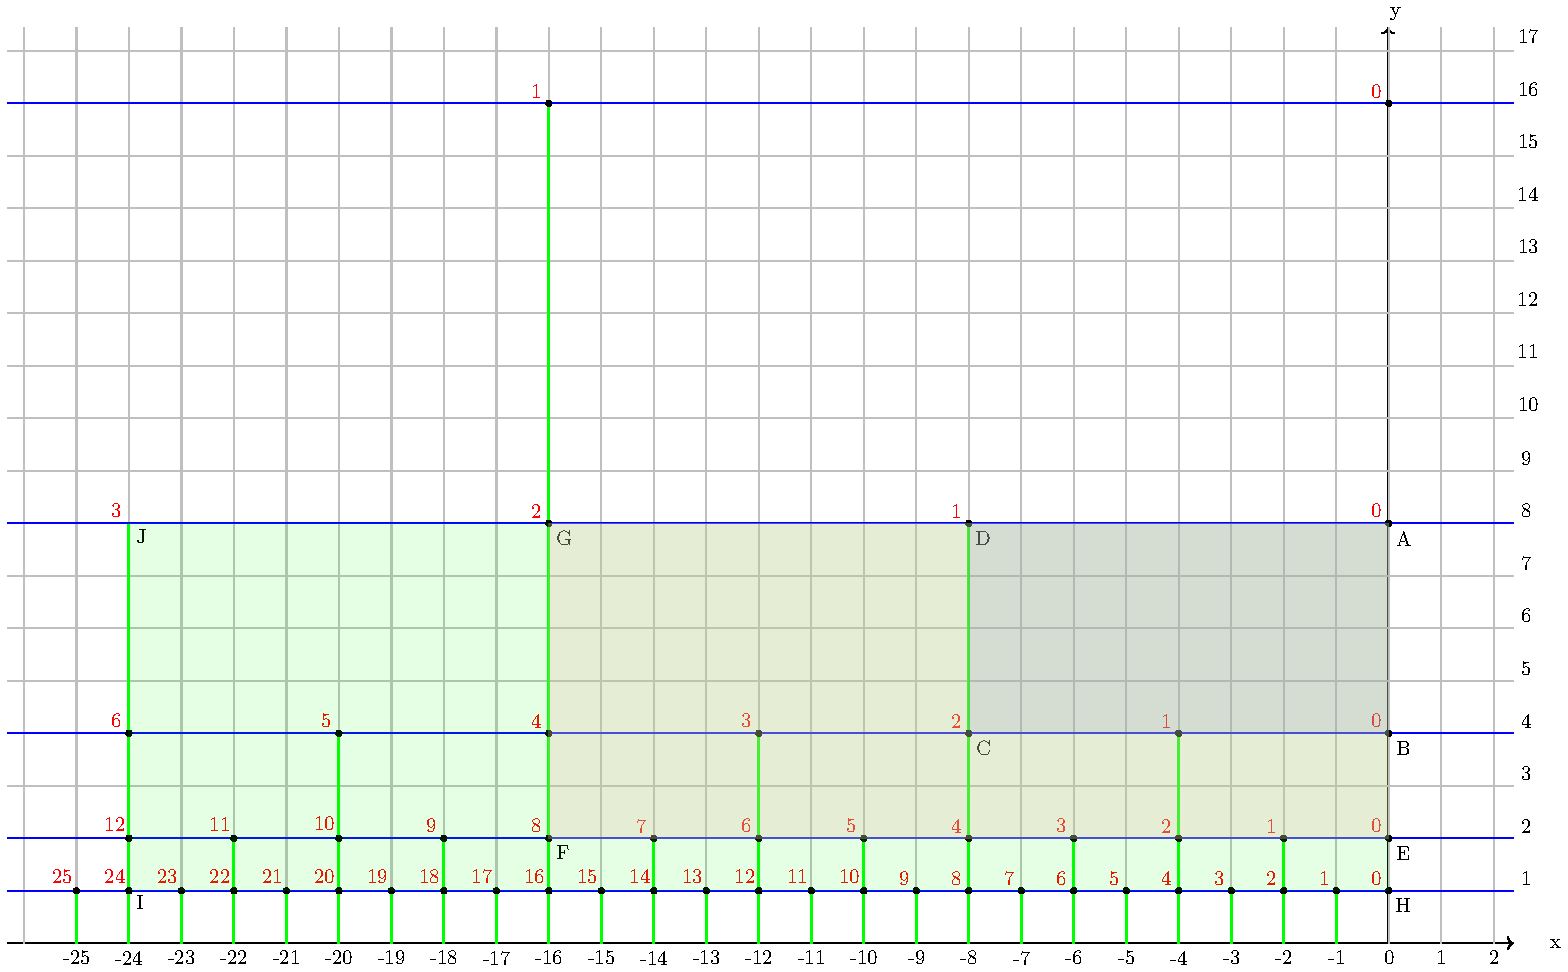
\includegraphics{images/17-area-formula}} % Use appropriate figure file
    \fbox{Placeholder for Figure: Torsion/Area Illustration}
    \caption{Illustration of the correspondence between accumulated arithmetic torsion (algebraic difference between paths) and the hyperbolic area (number of grid cells) enclosed by those paths in \( \mathfrak{E}_1(1, \ln 2) \).}
    \label{fig:area-formula_cs}
\end{figure}

This provides compelling macroscopic evidence within \( \mathfrak{E}_1 \) that \textbf{accumulated arithmetic torsion is proportional to the geometric area} enclosed by the corresponding evaluation paths on the grid.

The precise microscopic relationship was established by the differential formula derived from the flow equation (originally Eq~\eqref{eq:area_formula}):
\begin{equation}
    d\tau = \mu \lambda\, du\, dv \label{eq:area_formula_diff_cs}
\end{equation}
where \( d\tau \) is the infinitesimal torsion generated by commuting infinitesimal steps \( du \) (additive direction) and \( dv \) (multiplicative direction) in the local "arithmetic coordinate system". The term \( du\, dv \) represents the infinitesimal coordinate area element. This can be related to the geometric area element \( dS \) of the \( \mathfrak{E}_1 \) metric (via factors depending on the metric components in the \( u,v \) system, as in \( dS = |AB| du dv \)). This formula states that the local density of arithmetic torsion is directly proportional to \( \mu \lambda \) times the coordinate area density.

While we have macroscopic evidence (Figure~\ref{fig:area-formula_cs}) and the microscopic law (Equation~\eqref{eq:area_formula_diff_cs}), a rigorous \textbf{integral theorem} is still needed to bridge these scales. Such a theorem would formally relate the total torsion accumulated around a closed loop (or between two paths) to the integral of a torsion density (related to \( \mu \lambda \) and the metric) over the enclosed area, potentially involving boundary terms or curvature contributions, analogous to Green's theorem, Stokes' theorem, or the Gauss-Bonnet theorem in differential geometry. Formulating this integral connection remains a key area for future research.

Nevertheless, the results in \( \mathfrak{E}_1 \) strongly suggest that arithmetic torsion acts as a geometric measure of non-commutativity, akin to how curvature measures non-flatness. This space provides a concrete setting where algebraic structure translates directly into quantifiable geometric properties.


\section{The Tube Structure \( \mathcal{T} \) and Expression Dynamics} % (CS Section 6)

The preceding sections focused primarily on the geometry and properties of the first kind arithmetic expression space \( \mathfrak{E}_1(\mu, \lambda) \) for \emph{fixed} parameters \( \mu \) and \( \lambda \). However, arithmetic expressions often involve parameters, or we might be interested in how structures vary as the underlying operational strengths (\( \mu, \lambda \)) change. This necessitates extending our view from a single geometric space to a \emph{family} of spaces. This section introduces the concept of the "tube structure" \( \mathcal{T} \), which provides a framework for studying the dynamics of expressions across varying parameters, particularly focusing on the evolution of significant geometric features like zero loci.

\subsection{Family of Expression Spaces Indexed by \( \lambda \)} % (CS 6.1, from original 4.6.1/4.6.2)

Recall that the metric structure of \( \mathfrak{E}_1(\mu, \lambda) \), defined by Equation~\eqref{eq:metric_general_cs}, depends explicitly on the parameters \( \mu \) and \( \lambda \). While both parameters can vary, let us, for simplicity and concreteness in this initial exposition, fix the additive strength (e.g., \( \mu = 1 \)) and consider the family of spaces generated by varying the multiplicative strength parameter \( \lambda \). We denote the parameter space by \( \Lambda \), typically \( \Lambda = \mathbb{R}^+ \) (or some relevant interval).

For each \( \lambda \in \Lambda \), we have a specific geometric space:
\[
\mathfrak{E}_1^{(\lambda)} \coloneqq \mathfrak{E}_1(1, \lambda) = (\mathcal{B}, g_\lambda)
\]
where \( g_\lambda \) is the metric \( ds^2 = \frac{1}{y^2}(dx^2 + dy^2/\lambda^2) \) and the assignment function remains \( a(x,y) = -x/y \). We can think of this collection \( \{ \mathfrak{E}_1^{(\lambda)} \}_{\lambda \in \Lambda} \) as a family of related geometries.

Each individual space \( \mathfrak{E}_1^{(\lambda)} \) can be visualized as a "slice" or a "fiber" within this family. To study structures across these slices coherently, we introduce the concept of the total space encompassing the entire family.

\begin{definition}[Tube Structure \( \mathcal{T} \)]\label{def:tube_structure_cs}
The \textbf{tube structure} \( \mathcal{T} \) associated with the family \( \{ \mathfrak{E}_1^{(\lambda)} \}_{\lambda \in \Lambda} \) is the total space formed by these slices. Conceptually, it can be viewed as the disjoint union equipped with a suitable structure that relates the different fibers:
\[
\mathcal{T} = \bigsqcup_{\lambda \in \Lambda} \mathfrak{E}_1^{(\lambda)}
\]
Rigorously defining \( \mathcal{T} \) might involve specifying a topology, and potentially a smooth manifold or fiber bundle structure (e.g., viewing \( \mathcal{T} \) as a trivial bundle \( \Lambda \times \mathcal{B} \) with a \( \lambda \)-dependent metric). In this structure, \( \Lambda \) serves as the \textbf{base space}, and each \( \mathfrak{E}_1^{(\lambda)} \) is the \textbf{fiber} over the point \( \lambda \in \Lambda \).
\end{definition}

This tube structure provides the arena for studying how arithmetic-geometric objects behave as the fundamental parameter \( \lambda \) changes.

\subsection{Sections, Trajectories, and Zero Loci in \( \mathcal{T}_1 \)} % (CS 6.2, from original 4.6.2/4.6.3)

Within the tube structure \( \mathcal{T} \), we can track how specific arithmetic constructs manifest across the different \( \lambda \)-slices.

Consider a fixed algebraic structure, such as an alternating arithmetic path \( \alpha \) (Definition~\ref{def:alternating_path_cs}) whose operators \( \otimes_{\lambda_i}, \oplus_{\mu_i} \) might themselves depend on the external parameter \( \lambda \) in a prescribed way, or might be fixed relative to \( \lambda \). For example, a polynomial \( P(z) = \sum c_k z^k \) can be related to an arithmetic process involving \( \otimes_{\ln z} \). If we evaluate such a structure using the geometry corresponding to \( \lambda \), the result (e.g., the final assignment value, or the endpoint coordinates in \( \mathfrak{E}_1^{(\lambda)} \)) will depend on \( \lambda \).

As \( \lambda \) varies continuously in the base space \( \Lambda \), the point representing the evaluated structure in the corresponding fiber \( \mathfrak{E}_1^{(\lambda)} \) traces out a path within the total space \( \mathcal{T} \). Such a path, obtained by "lifting" a fixed algebraic entity into the \( \lambda \)-parameterized family of geometries, is called a \textbf{section} or a \( \lambda \)-trajectory through the tube structure. Studying the geometric properties of these sections (e.g., their smoothness, curvature within \( \mathcal{T} \)) is a potential avenue for research.

A particularly important structure to analyze within \( \mathcal{T} \) is the **zero locus** – the set of all points \( (\lambda, (x, y)) \in \mathcal{T} \) such that the assignment function evaluated in the corresponding slice is zero, i.e., \( a(x, y) = 0 \) within \( \mathfrak{E}_1^{(\lambda)} \).

Let \( \mathcal{T}_1 \) denote the tube structure built specifically from the family \( \{ \mathfrak{E}_1^{(\lambda)} \}_{\lambda \in \Lambda} \). In every slice \( \mathfrak{E}_1^{(\lambda)} \), the assignment function is \( a(x, y) = -x/y \). The condition \( a = 0 \) holds if and only if \( x = 0 \). This zero locus, the positive y-axis \( \{(0, y) \mid y > 0\} \subset \mathcal{B} \), is identical in every fiber \( \mathfrak{E}_1^{(\lambda)} \), irrespective of the value of \( \lambda \).

Consequently, the total zero locus within the tube \( \mathcal{T}_1 = \bigsqcup \mathfrak{E}_1^{(\lambda)} \) is simply the product set:
\[
\text{ZeroLocus}(\mathcal{T}_1) = \{ (\lambda, (x, y)) \in \Lambda \times \mathcal{B} \mid x = 0 \} \cong \Lambda \times \mathbb{R}^+
\]
This is a rather simple structure – a "vertical sheet" extending along the \( \lambda \)-dimension without any change in its cross-section within each fiber. The zero locus in the tube structure based on \( \mathfrak{E}_1 \) does \emph{not} exhibit any interesting evolution or dependence on the parameter \( \lambda \).

\subsection{Outlook: Nontrivial Tube Spaces and Topological Change} % (CS 6.3, from original 4.6.3/4.6.4)

The simplicity of the zero locus within \( \mathcal{T}_1 \) is a direct consequence of the rigid definition of the assignment function \( a = -x/y \) in the \( \mathfrak{E}_1 \) space. While \( \mathfrak{E}_1 \) provides a crucial foundational model demonstrating the core principles of AEG (satisfying the flow equation, torsion-area link), its fixed zero structure might limit its ability to model more complex arithmetic phenomena where parameter dependence plays a critical role (e.g., phenomena related to roots of polynomials depending on parameters, or perhaps analogies to knot invariants like the Alexander polynomial which depend on a variable).

This motivates the search for and construction of \textbf{"non-trivial" arithmetic expression spaces}, which we might denote \( \mathfrak{E}_{NT} \). Such spaces would differ from \( \mathfrak{E}_1 \) perhaps in their underlying manifold, their metric structure, or, more significantly, in their assignment function \( a_{NT}(x, y; \lambda) \), such that the zero locus \( a_{NT} = 0 \) within a single slice \( \mathfrak{E}_{NT}^{(\lambda)} \) could be more complex than just a single ray. For example, the zero locus might consist of multiple curves, or curves with self-intersections.

If such non-trivial spaces \( \mathfrak{E}_{NT}^{(\lambda)} \) exist and can be formed into a tube structure \( \mathcal{T}_{NT} = \bigsqcup \mathfrak{E}_{NT}^{(\lambda)} \), the total zero locus within \( \mathcal{T}_{NT} \) could exhibit rich and dynamic behavior as \( \lambda \) varies:
\begin{itemize}
    \item \textbf{Morphing/Evolution:} The shape, number, or position of the zero curves within the \( \lambda \)-slice could change continuously with \( \lambda \).
    \item \textbf{Bifurcation:} Zero loci could merge or split as \( \lambda \) crosses critical values, analogous to bifurcations in dynamical systems.
    \item \textbf{Topological Change:} The overall topology of the zero locus (viewed as a subspace within \( \mathcal{T}_{NT} \)) might change, potentially developing singularities, changing genus, or altering connectivity.
\end{itemize}
Analyzing these phenomena would require more advanced tools from differential geometry, topology, and singularity theory, applied within the AEG framework.

The construction and exploration of such non-trivial expression spaces and their associated tube structures represent a significant and necessary direction for future research. They hold the potential to connect AEG to deeper mathematical structures and to provide geometric tools for understanding parameter-dependent arithmetic systems, potentially linking to areas like algebraic geometry, number theory, and mathematical physics. The tube structure formalism, even in its initial form presented here, provides the conceptual language for framing these important investigations.

\section{Discussion and Future Directions} % (CS Section 7)

This paper has laid the initial groundwork for \emph{Arithmetic Expression Geometry} (AEG), a framework aiming to bridge the gap between the algebraic structure of arithmetic expressions and the continuous world of differential geometry. We began by reformulating threadlike expressions as paths governed by specific operators (Section~\ref{sec:paths_cs}), derived a fundamental Arithmetic Flow Equation linking these discrete operations to continuous propagation (Section~\ref{sec:flow_equation_cs}), and constructed the first concrete realization, the \( \mathfrak{E}_1 \) space, demonstrating its properties and hyperbolic nature (Section~\ref{sec:E1_space_cs}). We further explored geometric phenomena within \( \mathfrak{E}_1 \), including propagation dynamics, dual grid structures related to Baumslag–Solitar groups, and the compelling correspondence between arithmetic torsion and geometric area (Section~\ref{sec:propagation_grids_cs}). Finally, we introduced the tube structure \( \mathcal{T} \) as a means to analyze parameterized families of expression spaces (Section~\ref{sec:tube_structure_cs}).

This concluding section synthesizes these findings, discusses their broader implications and interpretations, and outlines several key avenues for future research that emerge from this foundational work.

\subsection{Summary of Findings and Significance}

The core contributions presented herein establish AEG as a viable and potentially fruitful research program:
\begin{itemize}
    \item \textbf{Geometric Formalism:} We provided a novel perspective, moving beyond purely syntactic or algebraic views to treat arithmetic expressions as geometric paths evolving within curved spaces.
    \item \textbf{Fundamental Dynamics:} The derived Arithmetic Flow Equation (\( \frac{da}{ds} = \mu \cos \theta + a \lambda \sin \theta \)) serves as a central dynamical law, intrinsically linking operational parameters (\( \mu, \lambda \)) and direction (\( \theta \)) to value propagation (\( da/ds \)). Its identification as an Eikonal/Hamilton-Jacobi equation connects AEG to established principles in physics and geometry.
    \item \textbf{Concrete Realization (\( \mathfrak{E}_1 \)):} The construction of the \( \mathfrak{E}_1 \) space on the upper half-plane provides a tangible hyperbolic setting where the theory is realized. The assignment function \( a = -x/y \) naturally satisfies the flow equation and, in the standard Poincaré case (\( \mu=1, \lambda=1 \)), possesses the significant property of being a Laplacian eigenfunction (eigenvalue -2, reflecting intrinsic hyperbolic structure).
    \item \textbf{Torsion as Area:} The demonstration within \( \mathfrak{E}_1 \) that arithmetic torsion (algebraic non-commutativity) corresponds quantitatively to enclosed hyperbolic area provides a powerful geometric interpretation of a fundamental algebraic phenomenon.
    \item \textbf{Parameter Dependence Framework:} The tube structure \( \mathcal{T} \) offers a conceptual framework for studying how expression geometry and dynamics depend on underlying parameters like \( \lambda \).
\end{itemize}
Collectively, these results suggest that a meaningful "geometry of computation" can be built directly from the structure of elementary arithmetic operations.

\subsection{Interpretations and Implications}

\paragraph{Arithmetic Torsion as Curvature.} The connection between arithmetic torsion and area in \( \mathfrak{E}_1 \) strongly suggests an analogy with curvature in differential geometry. Just as Gaussian curvature measures the deviation of a surface from being locally flat (Euclidean), arithmetic torsion measures the deviation of the combined arithmetic flow (\(\oplus_\mu, \otimes_\lambda\)) from being commutative. A non-zero torsion density \( d\tau/\frac{dS}{|AB|} = \mu \lambda |AB| \) indicates an intrinsic "arithmetic curvature" arising from the interplay between addition and multiplication. Exploring this analogy further – calculating integrated torsion, relating it to global properties – is a primary motivator for future work. Could different arithmetic systems (e.g., involving exponentiation) lead to different types of "curvature"?

\paragraph{A Geometric View of Computation?} If basic arithmetic operations possess inherent geometric structure, does this extend to more complex algorithms or computational processes? Can computational complexity or the properties of certain algorithms be understood through the lens of geometric invariants (like curvature, topology, or path lengths) in an appropriate AEG space? While speculative, this perspective offers a potentially new way to analyze computation.

\subsection{Future Directions and Open Problems}

This foundational work opens numerous avenues for further research:

\begin{enumerate}[label=\textbf{F\arabic*.}, leftmargin=*, widest=F6, align=left]
    \item \textbf{Integral Theorem for Torsion and Gauss-Bonnet Analogue:} A key theoretical goal is to formulate and prove an integral theorem that rigorously connects the microscopic torsion density \( d\tau = \mu \lambda du dv \) with the macroscopic accumulated torsion between paths or around loops in \( \mathfrak{E}_1 \) (and potentially other AEG spaces). Does this lead to a Gauss-Bonnet type theorem for AEG, relating integrated torsion/curvature to the topology of the expression domain or the boundary path properties?

    \item \textbf{Construction and Analysis of Non-Trivial Spaces (\( \mathfrak{E}_{NT} \)):} As highlighted in Section~\ref{sec:tube_structure_cs}, the \( \mathfrak{E}_1 \) space exhibits simple zero locus behavior. A crucial next step is to construct and investigate "non-trivial" AEG spaces (\( \mathfrak{E}_{NT} \)) where the assignment function or geometry allows for more complex zero sets (multiple curves, parameter-dependent shapes). Analyzing the dynamics within their tube structures (\( \mathcal{T}_{NT} \)), particularly the potential for bifurcation and topological change of zero loci as parameters vary, is essential for connecting AEG to richer mathematical phenomena.

    \item \textbf{Algebraic Classification of AEG Spaces:} The \( \mathfrak{E}_1 \) space revealed connections to Baumslag-Solitar groups. Can different AEG spaces be constructed based on different generating sets of arithmetic operations or different algebraic relations (e.g., corresponding to different groups or algebraic structures)? Can we develop a classification scheme for AEG spaces based on their underlying algebraic structure (groups, monoids, related presentations) and their geometric symmetry groups? How do the "Levels of Equality" discussed in the original draft (Section 2.6) influence the resulting geometry and its classification?

    \item \textbf{Connections to Other Mathematical Fields:}
        \begin{itemize}
            \item \textit{Geometric Group Theory:} Deepen the connection between AEG grid structures and the geometry of Cayley graphs, particularly for groups like BS(m,n), solvable groups, or perhaps hyperbolic groups. Can AEG provide new geometric models or insights for these groups?
            \item \textit{Knot Theory and Topology:} Explore potential links hinted at earlier. Can the evolution of zero loci in tube structures model invariants like the Alexander polynomial, known to arise from twisted homology related to non-abelian representations (often involving structures similar to \( BS(1, n) \))? Does the tube structure itself relate to fibrations?
            \item \textit{Number Theory and Modular Forms:} The appearance of hyperbolic geometry is suggestive. Are there specific AEG constructions related to number-theoretic functions, continued fractions, or modular groups acting on the upper half-plane?
            \item \textit{Logic and Computability:} Can the geometric perspective offer insights into the semantics of arithmetic, particularly concerning partiality (division by zero corresponding to geometric singularities?) or the decidability issues mentioned in Section~\ref{sec:paths_cs}? Does the geometry reflect different computational power or logical expressiveness?
        \end{itemize}

    \item \textbf{Global Metric Existence and Construction:} Resolve the open problem stated in Section~\ref{sec:flow_equation_cs} regarding the conditions under which a global metric can be found or constructed on a given manifold \( S \) such that a given function \( a: S \to \mathbb{R} \) satisfies the Arithmetic Flow Equation globally. This relates to global problems in geometric analysis (e.g., prescribing geometric quantities).

    \item \textbf{Higher Dimensions and Generalizations:} Extend the AEG framework to handle expressions with multiple variables (leading potentially to higher-dimensional AEG spaces) or different sets of operations (e.g., exponentiation, non-associative operations).
\end{enumerate}

\subsection{Concluding Remark}

Arithmetic Expression Geometry offers a nascent but potentially unifying perspective, weaving together threads from computation, algebra, and geometry. By treating arithmetic evaluation as a dynamic geometric process, AEG reveals unexpected structures like hyperbolic geometry emerging from basic operations, and provides quantitative links between algebraic properties like non-commutativity and geometric measures like area. The foundational \( \mathfrak{E}_1 \) space constructed and analyzed here serves as a crucial first step. The rich set of open problems and future directions suggests that further exploration of this geometry holds significant promise for uncovering deeper connections between the way we compute and the mathematical spaces that computation might naturally inhabit.

\newpage % Start appendices on a new page
\appendix % Starts appendix sections (labeled A, B, C...)

\section{Formal Solution of the Arithmetic Flow Equation} % (CS Appendix A)
\label{app:flow_solution}

This appendix provides the derivation of the formal solution to the Arithmetic Flow Equation~\eqref{eq:flow_cs}, assuming constant parameters \( \mu, \lambda \) and a constant direction angle \( \theta \). The equation is:
\[
\frac{da}{ds} = \mu \cos \theta + a \lambda \sin \theta
\]
This is a first-order linear non-homogeneous ordinary differential equation for \( a(s) \). We rewrite it in the standard form \( \frac{da}{ds} + P(s) a = Q(s) \):
\[
\frac{da}{ds} - (\lambda \sin \theta) a = \mu \cos \theta
\]
Here, \( P(s) = -\lambda \sin \theta \) and \( Q(s) = \mu \cos \theta \) are constants with respect to \( s \).

We solve this using an integrating factor \( I(s) \):
\[
I(s) = \exp\left( \int P(s) ds \right) = \exp\left( \int -\lambda \sin \theta \, ds \right) = e^{-\lambda s \sin \theta}
\]
Multiplying the standard form equation by \( I(s) \):
\[
e^{-\lambda s \sin \theta} \frac{da}{ds} - \lambda \sin \theta e^{-\lambda s \sin \theta} a = \mu \cos \theta e^{-\lambda s \sin \theta}
\]
The left-hand side is the derivative of the product \( a(s) I(s) \):
\[
\frac{d}{ds}\left( a e^{-\lambda s \sin \theta} \right) = \mu \cos \theta e^{-\lambda s \sin \theta}
\]
Integrating both sides with respect to \( s \):
\[
a e^{-\lambda s \sin \theta} = \int \mu \cos \theta e^{-\lambda s \sin \theta} ds
\]

We consider two cases for the integration:

\textbf{Case 1: \( \sin \theta \neq 0 \)} (i.e., \( \theta \) is not a multiple of \( \pi \))
\[
\int \mu \cos \theta e^{-\lambda s \sin \theta} ds = \mu \cos \theta \left( \frac{e^{-\lambda s \sin \theta}}{-\lambda \sin \theta} \right) + C_1
\]
where \( C_1 \) is the constant of integration. Substituting back:
\[
a e^{-\lambda s \sin \theta} = \frac{-\mu \cos \theta}{\lambda \sin \theta} e^{-\lambda s \sin \theta} + C_1
\]
Solving for \( a(s) \):
\[
a(s) = -\frac{\mu \cos \theta}{\lambda \sin \theta} + C_1 e^{\lambda s \sin \theta} = -\frac{\mu}{\lambda} \cot \theta + C_1 e^{\lambda s \sin \theta}
\]

\textbf{Case 2: \( \sin \theta = 0 \)} (i.e., \( \theta = k\pi \) for integer \( k \))
In this case, \( \cos \theta = \pm 1 \). The differential equation becomes \( \frac{da}{ds} = \mu (\pm 1) \). The integration is straightforward:
\[
a(s) = \pm \mu s + C_2
\]
This corresponds to pure addition (\( \theta = 0 \)) or subtraction (\( \theta = \pi \)).

Now, applying the initial condition \( a(0) = a_0 \) to the general solution (Case 1):
\[
a_0 = -\frac{\mu}{\lambda} \cot \theta + C_1 e^0 \implies C_1 = a_0 + \frac{\mu}{\lambda} \cot \theta
\]
Substituting \( C_1 \) back into the solution gives the final result presented in Equation~\eqref{eq:solution_cs}:
\begin{equation}
   a(s) = \left(a_0 + \frac{\mu}{\lambda} \cot \theta\right) e^{\lambda s \sin \theta} - \frac{\mu}{\lambda} \cot \theta \quad (\text{for } \sin \theta \neq 0) \label{eq:solution_appendix_cs}
\end{equation}
This solution also yields the correct limits for \( \theta \to 0 \) or \( \theta \to \pi \) corresponding to Case 2 (requires careful analysis using L'Hôpital's rule or Taylor expansion, consistent with the results found in Section~\ref{subsec:discrete-generating}). % Adjusted section reference


\section{Geometric Calculation Details for \( \mathfrak{E}_1 \)} % (CS Appendix B)
\label{app:geometry_calc}

This appendix provides supporting calculations for geometric properties discussed in the main text, particularly concerning the grid structures and torsion-area relationship within \( \mathfrak{E}_1 \).

\subsection{Grid Properties in \( \mathfrak{E}_1(1, \ln 2) \)}
\label{app:grid_properties}

We verify the orthogonality and unit length properties of the rectilinear grid (Figure~\ref{fig:grid1_cs}) within the space \( \mathfrak{E}_1(1, \ln 2) \), where \( \mu=1, \lambda=\ln 2 \). The metric is:
\[
ds^2 = \frac{1}{y^2}\left(dx^2 + \frac{dy^2}{(\ln 2)^2}\right)
\]
The inner product matrix is \( g = \text{diag}(1/y^2, 1/(y^2 (\ln 2)^2)) \).

\paragraph{Orthogonality.}
The tangent vector to a horizontal line (\(y=\text{const}\)) is \( \mathbf{t}_H = (1, 0) \).
The tangent vector to a vertical line (\(x=\text{const}\)) is \( \mathbf{t}_V = (0, 1) \).
Their inner product is:
\[
\mathbf{t}_H \cdot \mathbf{t}_V = g_{ij} t_H^i t_V^j = g_{xx}(1)(0) + g_{xy}(1)(1) + g_{yx}(0)(0) + g_{yy}(0)(1) = 0
\]
Thus, the horizontal and vertical coordinate lines are orthogonal under this metric.

\paragraph{Unit Length for +1 Step.}
A \( +1 \) operation corresponds to moving from \( a = -x/y \) to \( a+1 = -(x+\Delta x)/y \). This implies \( 1 = -\Delta x / y \), so \( \Delta x = -y \). The path is horizontal from \( (x, y) \) to \( (x-y, y) \). The arc length is:
\[
L_{+1} = \int_{x}^{x-y} \sqrt{ds^2} = \int_{x}^{x-y} \sqrt{\frac{1}{y^2}(dx^2 + 0)} = \int_{x}^{x-y} \frac{|dx|}{y} = \frac{1}{y} |(x-y) - x| = \frac{1}{y} |-y| = 1
\]

\paragraph{Unit Length for x2 Step.}
A \( \times 2 \) operation corresponds to moving from \( a = -x/y \) to \( 2a = -x/y' \). This implies \( 1/y' = 2/y \), so \( y' = y/2 \). The path is vertical from \( (x, y) \) to \( (x, y/2) \). The arc length is:
\[
L_{\times 2} = \int_{y}^{y/2} \sqrt{ds^2} = \int_{y}^{y/2} \sqrt{\frac{1}{y^2}(0 + \frac{dy^2}{(\ln 2)^2})} = \int_{y}^{y/2} \frac{|dy|}{y \ln 2}
\]
Since \( y > 0 \) and \( y/2 < y \), \( dy \) is negative, so \( |dy| = -dy \).
\[
L_{\times 2} = \int_{y/2}^{y} \frac{dy}{y \ln 2} = \frac{1}{\ln 2} [\ln y]_{y/2}^y = \frac{1}{\ln 2} (\ln y - \ln(y/2)) = \frac{1}{\ln 2} \ln\left(\frac{y}{y/2}\right) = \frac{\ln 2}{\ln 2} = 1
\]
These calculations confirm that the grid steps defined by \( +1 \) (horizontal) and \( \times 2 \) (vertical) have unit length with respect to the \( \mathfrak{E}_1(1, \ln 2) \) metric.

\subsection{Infinitesimal Arithmetic Torsion}
\label{app:infinitesimal_torsion}

We derive the formula \( d\tau = \mu \lambda \, du \, dv \) (Equation~\eqref{eq:area_formula_diff_cs}). Consider applying two infinitesimal steps: \( du \) in the \( \mu \)-direction and \( dv \) in the \( \lambda \)-direction, starting from value \( a \).
\begin{itemize}
    \item Path 1 (Add then Multiply): \( a \xrightarrow{\oplus_{\mu du}} a + \mu du \xrightarrow{\otimes_{\lambda dv}} (a + \mu du) e^{\lambda dv} \)
    \item Path 2 (Multiply then Add): \( a \xrightarrow{\otimes_{\lambda dv}} a e^{\lambda dv} \xrightarrow{\oplus_{\mu du}} a e^{\lambda dv} + \mu du \)
\end{itemize}
The infinitesimal torsion \( d\tau \) is the difference between the results of Path 1 and Path 2:
\[
d\tau = (a + \mu du) e^{\lambda dv} - (a e^{\lambda dv} + \mu du)
\]
Using the first-order Taylor expansion \( e^{\lambda dv} \approx 1 + \lambda dv \):
\begin{align*}
d\tau &\approx (a + \mu du) (1 + \lambda dv) - (a (1 + \lambda dv) + \mu du) \\
&= (a + a \lambda dv + \mu du + \mu \lambda du dv) - (a + a \lambda dv + \mu du) \\
&= \mu \lambda du dv
\end{align*}
This confirms the lowest-order contribution to the non-commutativity is proportional to the coordinate area element \( du dv \).

\subsection{Torsion Calculation for Grid Examples (Section~\ref{subsec:gridsandtorsion})} % Adjusted section reference
\label{app:grid_torsion_calc}

We verify the torsion values cited in Section~\ref{subsec:gridsandtorsion} for the \( \mathfrak{E}_1(1, \ln 2) \) grid (\(\mu=1, \lambda=\ln 2\), so ops are \(+1, \times 2\)). Torsion is calculated as the difference between applying a sequence of multiplications then additions versus applying the additions then the multiplications. Let \( \otimes^n \) denote \( n \) applications of \( \otimes_{\ln 2} \) (multiply by \( 2^n \)) and \( \oplus^m \) denote \( m \) applications of \( \oplus_1 \) (add \( m \)). We compare \( x \otimes^n \oplus^m \) and \( x \oplus^m \otimes^n \).

\paragraph{Case 1: n=1, m=1.} (\(\times 2, +1\))
\begin{itemize}
    \item Path 1 (\( \otimes \oplus \)): \( (x \otimes_{\ln 2}) \oplus_1 = 2x + 1 \)
    \item Path 2 (\( \oplus \otimes \)): \( (x \oplus_1) \otimes_{\ln 2} = (x+1) \times 2 = 2x + 2 \)
    \item Torsion = Path 1 Result - Path 2 Result = \( (2x+1) - (2x+2) = -1 \). (Matches area=1 with sign).
\end{itemize}

\paragraph{Case 2: n=2, m=2.} (\(\times 4, +2\))
\begin{itemize}
    \item Path 1 (\( \otimes^2 \oplus^2 \)): \( (x \otimes_{\ln 2} \otimes_{\ln 2}) \oplus_1 \oplus_1 = 4x + 1 + 1 = 4x + 2 \)
    \item Path 2 (\( \oplus^2 \otimes^2 \)): \( (x \oplus_1 \oplus_1) \otimes_{\ln 2} \otimes_{\ln 2} = (x+2) \times 2 \times 2 = (x+2) \times 4 = 4x + 8 \)
    \item Torsion = Path 1 Result - Path 2 Result = \( (4x+2) - (4x+8) = -6 \). (Matches area=6 with sign).
\end{itemize}

\paragraph{Case 3: n=3, m=3.} (\(\times 8, +3\))
\begin{itemize}
    \item Path 1 (\( \otimes^3 \oplus^3 \)): \( (x \otimes_{\ln 2}^3) \oplus_1^3 = 8x + 1 + 1 + 1 = 8x + 3 \)
    \item Path 2 (\( \oplus^3 \otimes^3 \)): \( (x \oplus_1^3) \otimes_{\ln 2}^3 = (x+3) \times 8 = 8x + 24 \)
    \item Torsion = Path 1 Result - Path 2 Result = \( (8x+3) - (8x+24) = -21 \). (Matches area=21 with sign).
\end{itemize}
These calculations confirm the numerical values used to illustrate the torsion-area relationship. The negative sign indicates the order difference consistently leads to a smaller value for the (Multiply first, Add second) path compared to the (Add first, Multiply second) path in these examples.


\section{Coordinate Transforms and Möbius Maps} % (CS Appendix C)
\label{app:coords_mobius}

This appendix details the relationship between the upper half-plane model \( \mathcal{B} \) and the Poincaré disk model \( \mathcal{P} \) used in Section~\ref{sec:E1_space_cs}, % Adjusted section reference
particularly concerning the horocycle coordinate system.

\subsection{Möbius Map: Upper Half-Plane to Poincaré Disk}
\label{app:mobius_map}

A standard conformal map \( f \) from the upper half-plane \( \mathcal{B} = \{ z = x+iy \mid y > 0 \} \) to the open unit disk \( \mathcal{P} = \{ w \in \mathbb{C} \mid |w| < 1 \} \) is given by:
\[
w = f(z) = \frac{z - i}{z + i}
\]
This map sends the reference point \( z=i \) (often considered the 'origin' of \( \mathcal{B} \)) to \( w=0 \) (the center of \( \mathcal{P} \)). It maps the real axis \( y=0 \) (the boundary of \( \mathcal{B} \), excluding \( \infty \)) to the unit circle \( |w|=1 \) (the boundary of \( \mathcal{P} \)). The point at infinity in \( \mathcal{B} \) maps to \( w=1 \).

The inverse map \( f^{-1}: \mathcal{P} \to \mathcal{B} \) is given by:
\[
z = f^{-1}(w) = i \frac{1 + w}{1 - w}
\]

\subsection{Horocycle Coordinates and Metric Equivalence}
\label{app:horocycle_coords}

We aim to show that the coordinate system \( (u, v) \) with metric \( ds^2 = e^{-2v} du^2 + dv^2 \) used in Section~\ref{subsec:horocycle_equiv_cs} % Adjusted section reference
is equivalent to the standard Poincaré metric \( ds^2 = (dx^2 + dy^2) / y^2 \) on \( \mathcal{B} \) under a suitable coordinate transformation.

Consider the transformation:
\begin{equation}
x = u, \quad y = e^v \label{eq:coord_transform_cs}
\end{equation}
This implies \( v = \ln y \). The differentials are \( dx = du \) and \( dy = e^v dv \).
Substituting these into the standard Poincaré metric on \( \mathcal{B} \):
\[
ds^2 = \frac{dx^2 + dy^2}{y^2} = \frac{(du)^2 + (e^v dv)^2}{(e^v)^2} = \frac{du^2 + e^{2v} dv^2}{e^{2v}} = e^{-2v} du^2 + dv^2
\]
This matches the metric form given in Equation~\eqref{eq:metric_horocycle_cs}. Therefore, the coordinates \( (u, v) \) defined by \( u=x, v=\ln y \) represent a valid coordinate system for the upper half-plane equipped with the standard Poincaré metric, where the metric takes the form \( e^{-2v} du^2 + dv^2 \). This specific coordinate system corresponds to horocycles centered at \( z = i \infty \) (which are horizontal lines \( y = e^v = \text{const} \) along which \( u=x \) varies) and orthogonal geodesics (which are vertical lines \( x=u=\text{const} \) along which \( v = \ln y \) varies).

Under this transformation~\eqref{eq:coord_transform_cs}, the assignment function \( a = -x/y \) becomes:
\[
a(u, v) = - \frac{u}{e^v} = -u e^{-v}
\]
This confirms the form of the assignment function used in the horocycle-based example (up to a sign, which relates to orientation choices).

\subsection{Laplacian Eigenvalue Convention}
\label{app:laplacian_convention}

As noted in Sections~\ref{sec:E1_space_cs} and \ref{app:horocycle_coords}, the calculated eigenvalue of the assignment function \( a \) under the Laplace-Beltrami operator differed between the \( (x, y) \) coordinates (using \( \Delta = -y^2(\partial_x^2 + \partial_y^2) \), yielding eigenvalue -2) and the \( (u, v) \) horocycle coordinates (using \( \Delta = e^{2v}\partial_u^2 + \partial_v^2 - \partial_v \), yielding eigenvalue +2).

This difference stems solely from the **convention** used in defining the Laplacian operator in each coordinate system. Geometricians often define \( \Delta = -\text{div} \circ \text{grad} \), which typically leads to non-positive eigenvalues for \( L^2 \) eigenfunctions on hyperbolic spaces. Other fields might use \( \Delta = \text{div} \circ \text{grad} \). The transformation between coordinate systems for the Laplacian is given by \( \Delta_w = |\frac{dz}{dw}|^2 \Delta_z \) only for conformal maps between *flat* spaces. For curved spaces, the intrinsic definition \( \text{div}(\text{grad} f) \) must be used, and its expression changes with the coordinate system and metric, potentially including lower-order terms (like the \( -\partial_v \) term in the horocycle case) and different overall scaling factors, which can affect the sign or value of the computed eigenvalue even for the same intrinsic operator.

The physically and geometrically significant fact is that the assignment function \( a \) \emph{is} an eigenfunction of the intrinsic Laplace-Beltrami operator in the standard \( \mathfrak{E}_1(1, 1) \) space. The specific numerical value (\(+2\) or \(-2\)) depends on the chosen coordinate system and the precise (sign) convention adopted for writing down the operator \( \Delta \) in those coordinates.


% --- Bibliography Commands ---
% \bibliographystyle{plain} % Or another style like amsplain, siam, etc.
% \bibliography{aeg-paper} % Your .bib file name

\end{document}